% ---------------------------------------------------------------------------
% Supplemental Material (S-numbered tables, figures and sections)
% ---------------------------------------------------------------------------
\setcounter{table}{0}
\setcounter{figure}{0}
\renewcommand{\thetable}{S\arabic{table}}
\renewcommand{\thefigure}{S\arabic{figure}}
\renewcommand{\thesection}{S\arabic{section}}
\renewcommand{\theHtable}{S\arabic{table}}
\renewcommand{\theHfigure}{S\arabic{figure}}
\renewcommand{\theHsection}{S\arabic{section}}

This Supplemental Material gives the data and benchmark settings, the details of the
commonality analysis of Sec.~\ref{sec:commonality}, and the full tables behind
Sec.~\ref{sec:results}. Every further number (the benchmarks scored by all-community
recovery, the selector and grid-edge diagnostics, the SNAP graphs on their induced
subgraphs and against distinct node sets, and every method's $\Omega$ and coverage on
the smaller real networks) is in the repository named in the main text, with the script
that produces it.

\section{Data}
\label{app:data}

Table~\ref{tab:data} lists the four networks with recorded memberships, and
Table~\ref{tab:datamore} the fourteen Netzschleuder networks of Table~\ref{tab:realmore}.
Groups of fewer than three nodes are discarded; the SNAP top-5000 lists repeat some node
sets, and $\Omega$ is scored against the distinct sets.

\begin{table}[h]
\caption{Networks with recorded memberships. Groups: the lines of the SNAP files
\texttt{all.cmty} (Amazon: \texttt{all.dedup.cmty}), as used in Sec.~\ref{sec:commonality};
detection is scored against the top-5000 lists, which repeat some node sets (1\,517
distinct sets for Amazon, 4\,961 for DBLP); $\Omega$ is scored against the distinct
sets. On YouTube detection is scored against every group of at least three nodes
(8\,385 groups on 47\,135 nodes). $f_{\rm lab}$: fraction of nodes with at least one
recorded membership.}
\label{tab:data}
\begin{ruledtabular}
\begin{tabular}{lrrrr}
Network & Nodes & Edges & Groups & $f_{\rm lab}$ \\
\hline
Karate club & 34 & 78 & 2 & 1.00 \\
DBLP & 317\,080 & 1\,049\,866 & 13\,477 & 0.82 \\
Amazon & 334\,863 & 925\,872 & 75\,149 & 0.95 \\
YouTube & 1\,134\,890 & 2\,987\,624 & 16\,386 & 0.046 \\
\end{tabular}
\end{ruledtabular}
\end{table}

\begin{table}[h]
\caption{The fourteen networks of Table~\ref{tab:realmore}: nodes, edges, recorded groups, and the fraction of nodes that carry at least one group; groups of fewer than three nodes are discarded. Political blogs includes 266 isolated nodes; the primary school network aggregates both days of contacts.}
\label{tab:datamore}
\begin{ruledtabular}
\begin{tabular}{lrrrr}
Network & Nodes & Edges & Groups & $f_{\rm lab}$ \\
\hline
College football & 115 & 613 & 12 & 1.00 \\
Political books & 105 & 441 & 3 & 1.00 \\
Political blogs & 1490 & 16715 & 2 & 1.00 \\
Primary school & 242 & 8317 & 10 & 0.96 \\
Facebook ego 0 & 333 & 2519 & 15 & 0.81 \\
Facebook ego 107 & 1034 & 26749 & 9 & 0.46 \\
Facebook ego 348 & 224 & 3192 & 14 & 0.97 \\
Facebook ego 414 & 150 & 1693 & 7 & 0.89 \\
Facebook ego 686 & 168 & 1656 & 14 & 1.00 \\
Facebook ego 698 & 61 & 270 & 8 & 0.84 \\
Facebook ego 1684 & 786 & 14024 & 15 & 0.97 \\
Facebook ego 1912 & 747 & 30025 & 39 & 0.95 \\
Facebook ego 3437 & 534 & 4813 & 18 & 0.18 \\
Facebook ego 3980 & 52 & 146 & 5 & 0.77 \\
\end{tabular}
\end{ruledtabular}
\end{table}


\section{Benchmark design, grids and settings}
\label{app:design}

Table~\ref{tab:shapes} lists the ring families, Table~\ref{tab:grids} the parameter grids
and Table~\ref{tab:doublebonds} the shared nodes and fused rings of the ring benchmarks.

\emph{Ring generator.} Rings are generated independently. The two nodes of each merged pair are drawn uniformly among all
nodes and redrawn when they lie on the same ring or either has already been merged; the
absorbed node's edges are moved to the survivor, so the graph has
$n_0-\lfloor o_n n_0\rfloor$ nodes, $\lfloor o_n n_0\rfloor$ of them in two rings. A
rewired edge keeps one endpoint, chosen at random, and moves the other to a non-neighbour
$w$ chosen either uniformly or preferentially, with probability proportional to
$(d_w+1)^\alpha$ under the current degrees ($\alpha=1$, linear; $\alpha=2$,
superlinear, which grows hubs); as $p\to1$ the planted structure is erased. The geometry
families rewire inside each ring before the merges and the noise, moving one endpoint of
each chosen edge to a uniformly random non-neighbour in the same ring; a control family
rewires by double-edge swaps inside each ring instead, which keeps every node's degree.
In the hub families each node draws its own even degree $k_i$ from a power law
$P(k)\propto k^{-2.5}$ on $\{k_r,\dots,8k_r\}$ and is joined to its $k_i/2$ nearest
neighbours on either side, so that communities keep their lattice neighbourhoods but
contain hubs. In the split-overlap families each of the two merged nodes first drops a
random half of its edges. Each random geometric community is a random geometric graph on
the unit torus with the size and mean degree of a ring, clustered (about $0.58$) but not
a lattice.

\emph{LFR graphs.} The reference implementation~\cite{lancichinetti2009benchmarks}
(\texttt{unweighted\_undirected}, compiled unmodified) with average degree
$\langle k\rangle=20$, maximum degree $k_{\max}=50$, degree and community-size exponents
$\tau_1=2$ and $\tau_2=1$, and community sizes between 20 and 100. The three slices at
$o_n=0.1$ use $\langle k\rangle=10$, $o_m=4$, and community sizes between 50 and 250,
respectively; the two clustered families, also at $o_n=0.1$, use the generator's
clustering option \texttt{-C} ($C_{\rm LFR}=0.3$, $0.5$).

\emph{Methods, software and settings.} Implementations are those of
\textsc{cdlib}~\cite{rossetti2019cdlib} (version 0.4.0),
\textsc{leidenalg}~\cite{traag_leidenalg} (0.11.0, with python-igraph 1.0.0),
\textsc{infomap}~\cite{edler_infomap} (2.10.1) and
\textsc{graph-tool}~\cite{peixoto_graphtool} (3.9), except SCAN and link communities,
which we implemented to expose the similarity and the cut, and OSLOM, the authors'
OSLOM2 code (\texttt{oslom\_undir}, unweighted); the stochastic block model and OSLOM
were run on the same graphs, checked edge for edge. We also use networkx 3.6.1,
numpy 2.4.1 and scipy 1.17.1. Leiden: iterated to convergence
(\texttt{n\_iterations}$=-1$), three restarts per resolution on the benchmarks and the
fourteen smaller networks, the restart kept being the one of highest objective value
under every protocol, so that no label enters the choice of restart, and one run per
resolution on Amazon, DBLP and YouTube; under the native protocol the L-CPM resolution
equals the edge density, at which the Constant Potts Model compares a group with an
Erd\H{o}s--R\'enyi graph of the same density~\cite{traag2011narrow}. Infomap:
two-level, one trial. Link communities: single linkage on closed-neighbourhood Jaccard,
cut at every value of HyperCommon's threshold grid, communities of fewer than three
nodes discarded; under the native protocol, cut where the partition density is largest
over the same grid, the criterion of Ref.~\cite{ahn2010link}. SCAN: cosine similarity on
closed neighbourhoods (SCAN-J: the same algorithm with Jaccard similarity); border nodes
reachable from several clusters are kept in all of them. Walktrap: walks of length 4,
dendrogram cut at maximum modularity (\textsc{cdlib}'s default). Stochastic block model:
run under Ubuntu (WSL), \texttt{minimize\_nested\_blockmodel\_dl} with default settings,
seeded from the graph seed (environment in \texttt{paper/environment-sbm.yml}).
Stochastic methods are seeded from the graph seed on the benchmarks, use five seeds on
the fourteen smaller networks (means reported) and one on Amazon, DBLP and YouTube.

\begin{table*}[tbp]
\caption{Ring-lattice families: rings of size $s$ and degree $k$, written
$(s,k)\times$count; $n_0=2000$ nodes before the merges, $o_n=0.05$ unless stated. All six
unequal families were also run at $o_n=0$ and $0.10$. Geometry families: uniform
$(50,8)\times40$, two worlds, three big, many small, and the gradient, each with a
fraction $q\in\{0,0.1,0.3,0.6,1\}$ of every ring's edges rewired inside the ring (one
endpoint moved), noise $p\in\{0,0.1,\dots,0.6\}$; the degree-preserving control uses
double-edge swaps on uniform $(50,8)\times40$ and three big, many small at
$q\in\{0.1,0.3\}$. Isolated-merge families: uniform $(50,8)\times40$ and
$(100,16)\times20$ at $o_n=0.01$, merges more than $2k$ apart on every ring,
$p\in\{0,0.05,0.1,0.2\}$. Hubs: $(50,k_i)\times40$ with $k_i\in\{4,\dots,32\}$,
$(100,k_i)\times20$ with $k_i\in\{8,\dots,64\}$, and two worlds with $k_i\in\{16,\dots,128\}$
on the five large rings and $\{4,\dots,32\}$ on the twenty small ones, $P(k_i)\propto
k_i^{-2.5}$ (mean degrees 9.2, 20.6 and 26.5). Split overlap: two worlds and three big,
many small at $o_n\in\{0.05,0.10\}$. Random geometric communities: the sizes and mean
degrees of uniform $(50,8)\times40$ and of two worlds. These control families use
$p\in\{0,0.1,\dots,0.8\}$. Null graphs: random geometric (2000 nodes, mean degree 8) and
Holme--Kim (2000 nodes, $m=4$, triangle probability $0.9$), $p=0$.}
\label{tab:shapes}
\begin{ruledtabular}
\begin{tabular}{ll}
Family & Rings \\
\hline
uniform & $(50,8)\times40$ or $(100,16)\times20$; $o_n\in\{0,0.05,0.10\}$ \\
two worlds & $(200,32)\times5$, $(50,8)\times20$ \\
three big, many small & $(400,32)\times3$, $(50,8)\times16$ \\
gradient & $(600,16)$, $(400,12)$, $(300,12)$, $(200,8)$, $(150,8)$, \\
 & $(120,8)$, $(100,8)$, $(60,8)$, $(40,8)$, $(30,8)$ \\
equal $k$, unequal $s$ & $(100,16)\times10$, $(50,16)\times20$ \\
 & $(100,8)\times10$, $(50,8)\times20$ \\
equal $s$, unequal $k$ & $(100,k)\times5$, $k\in\{32,24,16,8\}$ \\
preferential & uniform $(50,8)\times40$ and two worlds, $\alpha\in\{1,2\}$ \\
\end{tabular}
\end{ruledtabular}
\end{table*}

\begin{table*}[tbp]
\caption{Parameter grids (Sec.~\ref{sec:protocol}; the grids of clique percolation,
SLPA, DEMON, ANGEL and SCAN are the widened ones).
Logarithmically spaced grids list their end points and number of values. On Amazon,
DBLP and YouTube, Leiden's RB resolution runs over $\{0.01, 0.02, 0.05, 0.1, 0.25, 0.5,
1, 2, 4, 8, \dots, 4096\}$ (19 values, doubling from 1), its Constant Potts Model
resolution over 20 values from $10^{-5}$ to $0.5$, Infomap over the same Markov times
and the HyperCommon variants over the same $t$ grid; on Amazon and DBLP, link
communities also use the $t$ grid, and each commonality function 50 quantile levels of
its own triple scores. On the fourteen smaller networks the HyperCommon variants and
link communities search 100 quantile levels and the other methods the grids below; on
the benchmarks each commonality function searches 29 levels ($0,0.04,\dots,0.96$ and
$0.97,0.98,0.99,0.995$).}
\label{tab:grids}
\begin{ruledtabular}
\begin{tabular}{ll}
Method & Grid \\
\hline
HyperCommon, ablations, link communities & $t\in\{0.02,0.04,\dots,0.60\}$ (30) \\
Leiden, RB modularity & $\gamma$ from $1/16$ to $32$ (30, logarithmic), best of 3 restarts \\
Leiden, Constant Potts Model & $\gamma$ from $0.002$ to $0.5$ (30, logarithmic), best of 3 restarts \\
Infomap & Markov time from $0.25$ to $16$ (13, logarithmic) \\
CPM & clique size $\in\{3,\dots,7\}$ \\
SLPA & $r\in\{0.01,0.02,0.05,0.1,0.2,0.3,0.45\}$, 100 iterations \\
DEMON & $\epsilon\in\{0.1,0.25,0.5,0.75,0.9,1\}$ \\
ANGEL & threshold $\in\{0.1,0.25,0.5,0.75,0.9,1\}$ \\
SCAN (cosine) & $\epsilon\in\{0.1,\dots,0.8\}$, $\mu_{\rm SCAN}\in\{2,3,5\}$ \\
SCAN (Jaccard) & $\epsilon\in\{0.1,\dots,0.6\}$, $\mu_{\rm SCAN}\in\{2,3,5\}$ \\
Walktrap & walks of length 4, dendrogram cut at maximum modularity \\
label propagation & parameter-free \\
stochastic block model & level of the nested hierarchy (finest first; 1--6 levels with more than one group) \\
OSLOM & $t\in\{10^{-14},10^{-11},10^{-8},10^{-5},10^{-2},0.1\}$, otherwise its defaults (10 runs, first level) \\
\end{tabular}
\end{ruledtabular}
\end{table*}

\begin{table}[t]
\caption{Shared pairs in the ring benchmarks without noise (mean over ten graphs): merges, ring pairs sharing at least one node, ring pairs sharing two merged nodes within ring distance $k$ on both rings (Proposition~\ref{prop:sharedpairs}), the share of rings in such a pair, and the share of rings that exact HyperCommon fuses with another ring just above the lower edge $1/(2k_{\min}+1)$ of the recovery window (a detected community holding at least three unshared nodes of each of two rings; analysis/double\_bonds.py).}
\label{tab:doublebonds}
\scriptsize\setlength{\tabcolsep}{2pt}
\begin{ruledtabular}
\begin{tabular}{lcrrrrr}
Family & $o_n$ & merges & sharing & pair & rings & fused \\
\hline
uniform $(50,8)$ & 0.05 & 100 & 94.2 & 0.8 & 0.04 & 0.11 \\
uniform $(50,8)$ & 0.10 & 200 & 180.0 & 2.2 & 0.11 & 0.38 \\
uniform $(100,16)$ & 0.05 & 100 & 77.2 & 2.6 & 0.24 & 0.61 \\
uniform $(100,16)$ & 0.10 & 200 & 126.9 & 8.7 & 0.61 & 1.00 \\
two worlds & 0.05 & 100 & 74.7 & 3.8 & 0.22 & 0.35 \\
three big, many small & 0.05 & 100 & 51.7 & 3.8 & 0.25 & 0.40 \\
gradient & 0.05 & 100 & 27.5 & 1.2 & 0.20 & 0.37 \\
equal $k$, unequal $s$ ($k{=}16$) & 0.05 & 100 & 86.8 & 2.8 & 0.17 & 0.42 \\
equal $k$, unequal $s$ ($k{=}8$) & 0.05 & 100 & 88.7 & 0.3 & 0.02 & 0.06 \\
equal $s$, unequal $k$ & 0.05 & 100 & 79.3 & 3.0 & 0.25 & 0.54 \\
two worlds & 0.10 & 200 & 117.6 & 11.7 & 0.43 & 0.75 \\
three big, many small & 0.10 & 200 & 74.6 & 8.8 & 0.47 & 0.81 \\
gradient & 0.10 & 200 & 34.3 & 5.0 & 0.53 & 0.75 \\
equal $k$, unequal $s$ ($k{=}8$) & 0.10 & 200 & 153.1 & 2.5 & 0.16 & 0.42 \\
equal $k$, unequal $s$ ($k{=}16$) & 0.10 & 200 & 154.6 & 9.6 & 0.50 & 0.95 \\
equal $s$, unequal $k$ & 0.10 & 200 & 124.0 & 12.2 & 0.68 & 0.98 \\
\end{tabular}
\end{ruledtabular}
\end{table}


\clearpage

\section{Further proofs and details of the theory}
\label{app:proofsmore}

This section completes Appendix~\ref{app:proofs} of the main text.

\subsection{The two ends of the hierarchy}

With the counts $c_{\mathcal C}(i,j)$ and pair fractions $\pi_{\mathcal C}(c)$ of the
Omega index (Sec.~\ref{sec:metrics}):

\begin{lemma}
\label{lem:constant}
If $c_{\mathcal C}(i,j)=c$ for every pair and $c_{\mathcal G}$ is not identically $c$,
then $\Omega=0$.
\end{lemma}

\begin{proposition}[Endpoints]
\label{prop:endpoints}
Let the ground truth give some pair count $0$ and some pair count $\ge1$.
(i) If $G$ is connected and $|V|\ge3$, then $\mathcal C_0=\{V\}$ and $\Omega(0)=0$.
(ii) The communities at $t=1$ are the classes of nodes with identical closed
neighbourhoods having at least three members; if there are none,
$\mathcal C_1=\varnothing$ and $\Omega(1)=0$.
Consequently, when both hold, whenever $\Omega(t)>0$ for some $t$ the maximum
$\Omega^\star=\max_t\Omega(t)$ is attained at an interior threshold $t^\star\in(0,1)$.
\end{proposition}
The proposition does not assert that $\Omega^\star>0$ or that $\Omega(t)$ has a single
maximum; both are empirical. On noise-free ring lattices (ii) holds when $s\ge2k+2$, and
(i) when the merges connect all rings, which random merges usually do.

\begin{proof}[Proof of Lemma~\ref{lem:constant}]
$\pi_{\mathcal C}$ is concentrated on $c$, so $\Omega_e=\pi_{\mathcal G}(c)<1$; a pair agrees
exactly when $c_{\mathcal G}(i,j)=c$, so $\Omega_u=\pi_{\mathcal G}(c)$ as well.
\end{proof}

\begin{proof}[Proof of Proposition~\ref{prop:endpoints}]
(i) At $t=0$ every wedge is admissible. Two edges sharing an endpoint form a wedge, and
the wedges built on a common edge share its endpoints, so a walk in the line graph of
$G$ is a walk in $L_0$. The line graph of a connected graph is connected, and every
node of a connected graph with $|V|\ge3$ lies on a wedge. The single community $V$
gives $c_{\mathcal C}\equiv1$, and Lemma~\ref{lem:constant} applies.
(ii) $J(u,v)=1$ iff $N[u]=N[v]$, an equivalence relation whose classes are cliques; a
triple is admissible at $t=1$ iff it lies within one class, and triples within one
class are connected in $L_1$. Without classes of size at least three, $c_{\mathcal C}\equiv0$
and Lemma~\ref{lem:constant} applies. For the final claim: the cover changes only at
the finitely many distinct triple scores, so $\Omega(t)$ takes finitely many values on
$[0,1]$ and its maximum $\Omega^\star$ is attained; under the stated hypotheses
$\Omega(0)=\Omega(1)=0$ by (i) and (ii), so since $\Omega^\star\ge\Omega(t)>0$ every
maximiser lies in $(0,1)$.
\end{proof}

\subsection{Further ring-lattice windows}

\emph{Smaller rings and multiple merges.} For a single merge between two rings, exact
computation for $k=4$ to $12$ shows that the window of Eq.~\eqref{eq:window} also holds
for ring sizes down to $s=k+4$ for $k=4$ and $6$, and $s=k+2$ for $k=8$ to $12$; smaller
rings widen it upward (for $k=4$ and $s=6$ or $7$ it is $(1/9,2/5]$), which covers the
rings of Fig.~\ref{fig:schematic}. A node formed by merging one node from each of $m$
rings (all other merges isolated) gives the window
$(1/(2k+1),\min\{k/(mk+2),\max((k-2)/(k+4),(k-1)/(mk+3))\}]$, whose upper edge tends to
$1/m$ as $k$ grows; it is non-empty if and only if $m\le2k$. These statements and
Eqs.~\eqref{eq:window} and~\eqref{eq:windowab} were checked in rational arithmetic at
and on either side of every distinct commonality value (analysis/exact\_windows.py).

\emph{Unequal degrees.} For one isolated merge between rings of even degrees
$k_a,k_b\ge4$ and sizes at least $2k_a+2$ and $2k_b+2$, the same argument applies with
the commonalities of Lemma~\ref{lem:ringJ} for unequal degrees: with $x,z$ on the ring
of degree $k_a$, $J_u(d)=(k_a+1-d)/(k_a+k_b+1+d)$ and $J(z,y')=1/(k_a+k_b+1)$. The cross
pair has
$J=1/(k_a+k_b+1)$, which gives the lower edge of Eq.~\eqref{eq:windowab}. On the ring of
degree $x$, with $y$ the degree of the other ring, the upper-edge argument runs with
$J_u(1)=x/(x+y+2)$, $J_u(2)=(x-1)/(x+y+3)$ and $J(3)=(x-2)/(x+4)$, which gives
$U(x,y)$; both rings must be recovered, which gives the minimum over $U(k_a,k_b)$ and
$U(k_b,k_a)$.

\emph{Obstruction for unequal degrees.} A shared node between a dense and a sparse
community is held more weakly by the sparse one, so the window of such a merge narrows
and moves down, with upper edge $k_b/(k_a+k_b+2)$ for $k_a\gg k_b$. It cannot overlap
the window of merges between two sparse rings, whose lower edge is $1/(2k_b+1)$, once
$k_a\ge2k_b^2-2$: beyond that degree contrast no single threshold recovers a family that
also contains merges between two sparse rings, even without noise.
\subsection{Fusion of rings through shared pairs}

\emph{Fusion of rings.} Connectivity through shared pairs is what lets a community grow
through its own open wedges, and Proposition~\ref{prop:sharedpairs} is its counterpart.
On ring lattices, three communities that pairwise share single
nodes are joined when two of the three shared-node pairs are adjacent and the third lies
within distance $k$; for $k=8$ and pairwise adjacent shared nodes two apart, the rings
are recovered only for $4/13<t\le4/9$, and for $k=4$ they are never recovered. Two rings
joined only through two shared merged nodes, with no other merge within ring distance
$k$ of them, can be fused above the lower edge $1/(2k+1)$ only when those nodes lie
within ring distance $k$ of each other on both rings, or within $k/2$ on one ring and
within $3k/2$ on the other; for $k=8$, shared nodes $2$ apart on one ring and $11$ apart
on the other fuse the rings for $t\le3/23$. Theorem~\ref{thm:window}'s isolation
hypothesis excludes both cases. Whether fusion then occurs depends on the threshold,
since the merge lowers the commonality of the shared pair: two rings with $s=50$, $k=8$
that share two nodes four positions apart are fused at small $t$ but recovered
separately at $t=0.4$, where the shared pair, with $J=1/3$, is not admitted.

\subsection{Cost}

Every commonality needed is available from the wedges themselves: for a pair $\{a,b\}$,
$|N[a]\cap N[b]|$ is the number of common neighbours of $a$ and $b$, that is of centred
wedges $a$--$c$--$b$ (a triangle contributes once to each of its three pairs), plus $2$
if $a\sim b$, so one pass over the centred wedges, with pairs indexed by hashing, counts
all of them. Our implementation finds components on the incidence graph between admitted
triples and their pairs over a grid of thresholds. Alternatively, as in sequential clique
percolation~\cite{kumpula2008sequential}, a single union--find sweep over the triples in
decreasing order of score builds the merge tree of the triple components at all
thresholds in $O(W\log W)$, from which the cover at any one threshold is read in $O(W)$
more. For heavy-tailed degree distributions the hubs dominate through $W$, as for
every triangle-based method.

\emph{Degree-ratio pruning.} In the pruning of Sec.~\ref{sec:cost}, every wedge through
an edge with $\rho<t_{\min}$ is discarded. Common neighbours reached through discarded
edges must still be counted, for example by intersecting the adjacency lists of the kept
pairs; counting only the kept wedges would underestimate $J$. This is the size filter of
exact set-similarity joins~\cite{arasu2006efficient,bayardo2007scaling}, applied to
closed neighbourhoods of sizes $d_u+1$ and $d_v+1$. The pruning applies to every rule
that tests the edges of a wedge, including our three ablations, but not to link
communities, which score a wedge by its non-adjacent pair alone, whose commonality is
not bounded by the degrees of the wedge's edges, so every wedge through a hub has to be
enumerated. Our implementation counts the common neighbours of the kept pairs from the
full adjacency matrix, and pruned and unpruned runs give identical covers on its test
graphs, which include a hub joined to many leaves, and on the full Amazon and DBLP graphs
at all 30 thresholds $t\ge0.02$ of our grid.


\clearpage

\section{Commonality in empirical networks}
% Material moved from Sec. III (commonality in empirical networks) of the main text.
\subsection*{Commonality in empirical networks: details}

\emph{Unlabelled nodes.} Edges touching unlabelled DBLP authors join low-degree nodes in
small, tightly knit groups -- the median larger endpoint degree of the pooled
``different'' class is 8, against 22 for same-venue edges -- and have high commonality
(median $J=0.40$); pooled into the ``different'' class they push its median above that
of same-venue pairs, and the AUC for separating the classes falls to $0.41$
[Fig.~\ref{fig:S-realcommonality}(f)]. Even after unlabelled edges are set apart,
``outer'' means no recorded shared group, not proven separation: on the same DBLP
co-authorship network with venue groups, and on an Amazon co-purchasing network with
product-category groups, standard methods recover the recorded groups
poorly~\cite{hric2014community}. With unlabelled edges set apart, the inner and outer
medians of closed-neighbourhood Jaccard are $0.29$ and $0.15$ in the karate club, $0.25$
and $0.17$ in DBLP, $0.27$ and $0.20$ in Amazon, and $0.032$ and $0.022$ in YouTube
[Fig.~\ref{fig:S-realcommonality}(a--d)].

\emph{Degree strata.} The stratum AUCs of Amazon and YouTube lie around their pooled
$0.60$ and $0.61$ [Fig.~\ref{fig:S-realcommonality}(g,h)]. Their weaker signal is
consistent with what their ground truth is: Amazon's product categories are nested, with
95\% of labelled products in several categories, and YouTube's groups are user-declared
interests rather than structural units~\cite{yang2015defining}.

\emph{The family of functions.} With $I=|N[u]\cap N[v]|$ and $U=|N[u]\cup N[v]|$, the
eight functions of Fig.~\ref{fig:realfamily} are the raw overlap $I$; Jaccard
$I/U$~\cite{jaccard1912distribution}; the generalisations $I^2/U$ and $I/U^{1/2}$ of the
form $I^a/U^b$ (the first ranks pairs as the degree-normalised score
$I^2/(\langle d\rangle U)$ of Ref.~\cite{deinega2023thesis}, and the two rank pairs
identically, since $I/U^{1/2}=(I^2/U)^{1/2}$, so they count as one choice for any
threshold-based use); the cosine $I/\sqrt{|N[u]||N[v]|}$~\cite{salton1983introduction}
used by SCAN~\cite{xu2007scan}; the overlap normalised by the smaller and by the larger
neighbourhood, $I/\min$ and $I/\max$ (closed-neighbourhood versions of the hub-promoted
and hub-depressed indices~\cite{zhou2009predicting,lu2011link}, the first derived from
the topological overlap of Ravasz \emph{et al.}~\cite{ravasz2002hierarchical}); and, as a
structurally different score, resource allocation~\cite{zhou2009predicting}
$\sum_{w\in N(u)\cap N(v)}1/d_w$, which weights shared neighbours by their rarity. The
karate club is too small to stratify; there every function separates the classes in
aggregate, with AUC $0.73$--$0.89$. That the overlap-based scores perform alike within
strata is expected, since the strata are narrow degree bins. Commonality is therefore
best understood as a family whose appropriate member depends on the network.

\emph{Pairs and triples.} We sample wedges whose three nodes are labelled and weight
closed triangles by $1/3$, so that the population is unique triples rather than centred
wedges. The pair rule tests two pairs for an open wedge and three for a triangle;
Fig.~\ref{fig:realtriples} compares the two rules over the full range of thresholds. At
recall $0.2$, $91\%$ of pair-admitted triples are pure against $92\%$ of triple-admitted
ones in Amazon (base rate $86\%$), and $10\%$ against $13\%$ in YouTube (base rate
$10\%$). Closed triangles alone are $99\%$ pure in DBLP, reflecting cliques of
co-authors, but cover only a quarter of the pure triples; open wedges supply the rest,
which is the trade-off the triple rule manages.

\begin{figure*}[p]
  \centering
  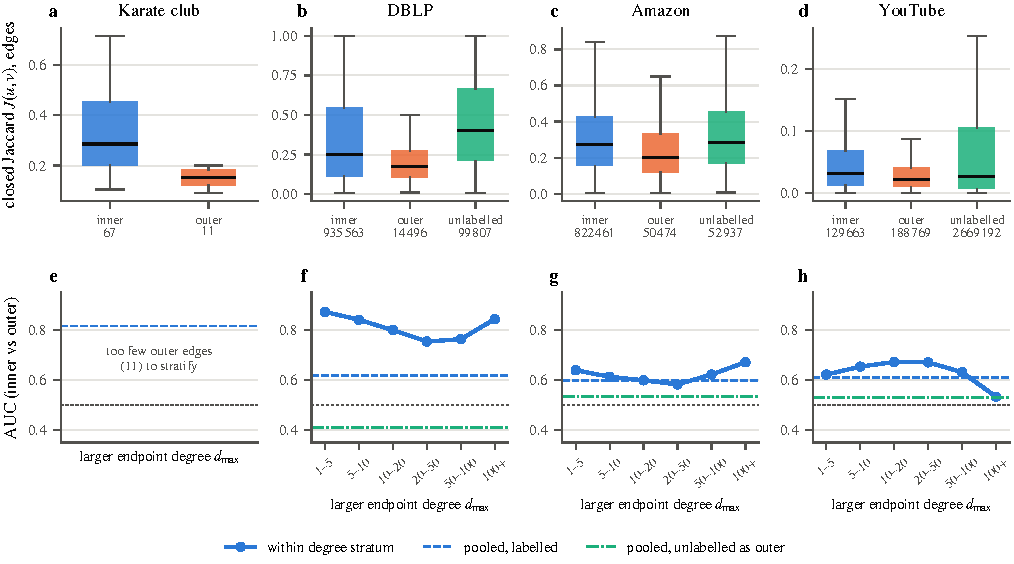
\includegraphics[width=\textwidth]{figures/fig_real_commonality.pdf}
  \caption{Commonality of edges in four networks with recorded memberships.
  (a--d)~Closed-neighbourhood Jaccard of edges whose endpoints share a recorded group
  (inner), are both labelled but share none (outer), or include an unlabelled node;
  boxes span the quartiles, whiskers the 5th--95th percentiles, numbers give edge
  counts. (e--h)~AUC for separating inner from outer edges within strata of the larger
  endpoint degree (points), pooled over all labelled edges (dashed), and with
  unlabelled edges counted as outer (dash-dotted), as in the earlier analysis of
  Ref.~\cite{deinega2023thesis}.}
  \label{fig:S-realcommonality}
\end{figure*}

\begin{figure*}[p]
  \centering
  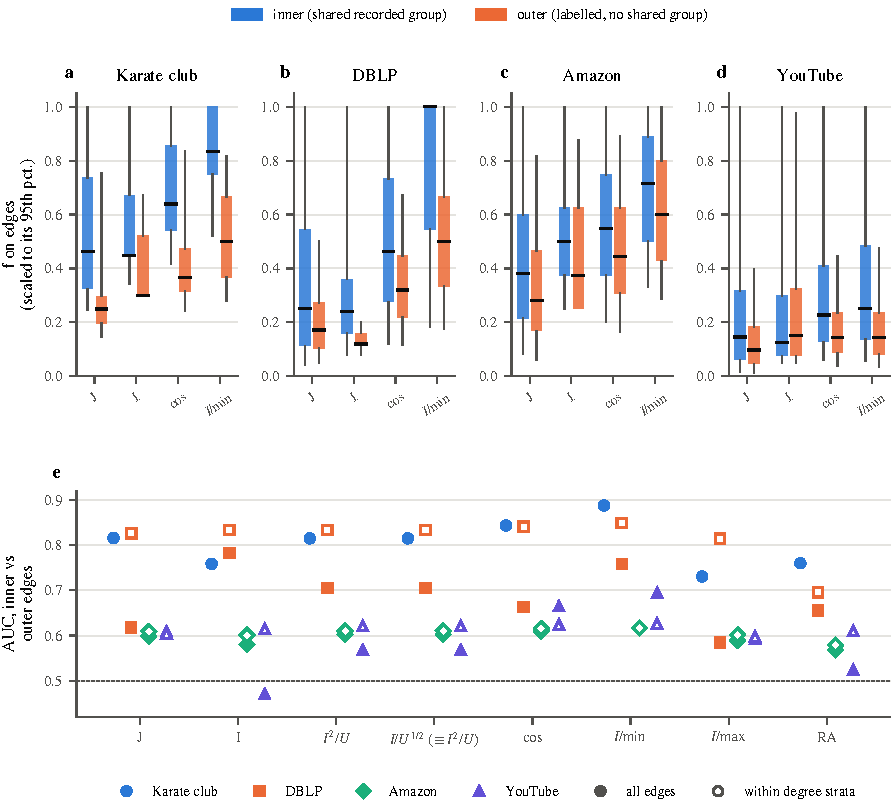
\includegraphics[width=\textwidth]{figures/fig_real_family.pdf}
  \caption{Commonality as a family of functions. (a--d)~Inner (shared recorded group)
  and outer (labelled, no shared group) edges under four functions, each scaled to its
  own 95th percentile. (e)~AUC for separating inner from outer edges with eight scores,
  over all labelled edges (filled) and within strata of both endpoint degrees (open);
  $I/U^{1/2}$ ranks pairs as $I^2/U$ does. The karate club is too small to stratify.}
  \label{fig:realfamily}
\end{figure*}

\begin{figure*}[p]
  \centering
  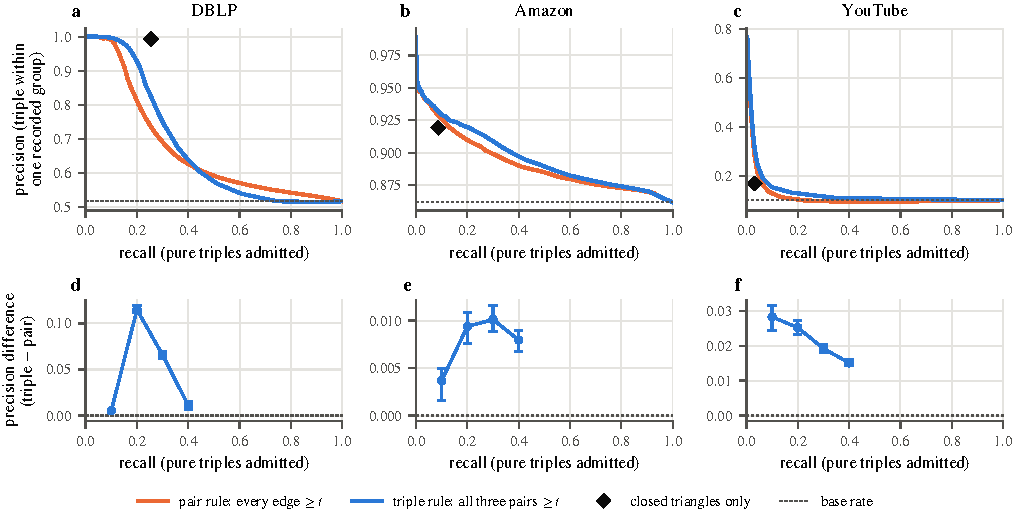
\includegraphics[width=\textwidth]{figures/fig_real_triples.pdf}
  \caption{Pair rule versus triple rule on unique labelled triples (wedges sampled
  uniformly, triangles weighted $1/3$). Precision is the fraction of admitted triples
  contained in one recorded group, recall the fraction of such triples admitted, as
  the threshold varies. Diamond: closed triangles only, without a threshold. Bottom
  row: difference in precision between the triple and the pair rule at equal recall,
  with 95\% intervals from resampling the triples; the y-axes of the top row differ
  between panels.}
  \label{fig:realtriples}
\end{figure*}

\clearpage

\section{Benchmarks}
% ---------------------------------------------------------------------------
% Supplemental Material: details behind Sec. VII (Results) of the main text
% ---------------------------------------------------------------------------

This section gives the full benchmark tables behind Sec.~\ref{sec:results} and the
details the main text summarises. Numbers quoted for a ring family without its overlap
level are at $o_n=0.05$.

\emph{Recovery window and fusions.} At $o_n=0.05$, for $k=16$ the isolation hypothesis
of Theorem~\ref{thm:window} cannot hold, and for $k=8$ it would need exactly five merge
positions more than $k$ apart on every ring. Rings are then fused inside the window in
three ways: two rings share two merged nodes within ring distance $k$ on both rings
(Proposition~\ref{prop:sharedpairs}); they share two merged nodes within $k/2$ on one
ring and within $3k/2$ on the other; or the merged nodes of three pairwise-merged rings
form an admissible wedge. Without noise, between $6\%$ and $61\%$ of the rings of a family
are fused at $o_n=0.05$ and between $38\%$ and all of them at $o_n=0.10$
(Table~\ref{tab:doublebonds}). For $k=16$ the noise-free curve of
Fig.~\ref{fig:omegat}(b) reaches $0.95$ only for $t\ge0.30$.

\begin{table*}[t]
\caption{Accuracy on the benchmarks as a user would run the methods, every parameter chosen without labels by one rule: on each test graph, the parameter whose cover has the largest overlapping modularity, Eq.~\eqref{eq:qov}, which for a partition is the Newman--Girvan modularity (label-free protocol). $\Omega$, mean over the noise range ($p\in[0,0.8]$ for rings, $\mu\in[0.1,0.6]$ for LFR), ten test graphs per noise level. HC: HyperCommon; e-c.: its triples joined only through shared edges; tri.: triangles only (J-thresholded 3-clique percolation~\cite{palla2005uncovering,kumpula2008sequential}); 2-test: third pair not tested; Link: link communities with the same similarity; CPM: clique percolation; Leiden: Leiden with the Reichardt--Bornholdt modularity; L-CPM: Leiden with the Constant Potts Model; Info.: Infomap; Walk.: Walktrap, walks of length 4, dendrogram cut at maximum modularity; LPA: label propagation; SBM: nested degree-corrected stochastic block model, each level of its hierarchy a parameter value; OSLOM: order statistics local optimisation, significance threshold $t$ as its parameter; SCAN: SCAN with cosine similarity; SCAN-J: SCAN with Jaccard similarity; $\alpha$: exponent of the preferential (degree-biased) noise. Parameter-free methods (Walktrap, LPA) are as under every protocol. Superscripts on HC: the paired 95\% bootstrap interval of its difference from the best other method (ablations excluded) lies above zero ($+$), contains zero ($=$) or lies below zero ($-$). Bold: best in row, within 0.005. 95\% bootstrap half-widths of these means over the ten test seeds have median 0.007 and maximum 0.050.}
\label{tab:labelfree}
\scriptsize\setlength{\tabcolsep}{1.35pt}
\resizebox{\textwidth}{!}{%
\begin{tabular}{llcccc|cc|cccccc|cccccc}
\hline\hline
 & & \multicolumn{4}{c}{HC and ablations} & \multicolumn{2}{c}{relatives} &\multicolumn{6}{c}{partitions} & \multicolumn{6}{c}{overlapping methods} \\
Family & $o_n$ & HC & e-c. & tri. & 2-test & Link & CPM & Leiden & L-CPM & Info. & Walk. & LPA & SBM & SLPA & OSLOM & DEMON & ANGEL & SCAN & SCAN-J \\
\hline
uniform, $k{=}8$ & 0.00 & \textbf{0.61$^{=}$} & \textbf{0.61} & 0.51 & 0.51 & 0.60 & 0.51 & \textbf{0.61} & \textbf{0.61} & 0.48 & 0.39 & 0.14 & 0.38 & 0.36 & 0.55 & 0.53 & 0.52 & 0.50 & 0.53 \\
 & 0.05 & \textbf{0.55$^{+}$} & 0.54 & 0.49 & 0.29 & 0.53 & 0.49 & 0.44 & 0.43 & 0.32 & 0.24 & 0.12 & 0.27 & 0.33 & 0.45 & 0.44 & 0.39 & 0.26 & 0.30 \\
 & 0.10 & \textbf{0.50$^{+}$} & \textbf{0.50} & 0.46 & 0.22 & 0.45 & 0.44 & 0.32 & 0.31 & 0.25 & 0.18 & 0.11 & 0.21 & 0.30 & 0.37 & 0.40 & 0.40 & 0.21 & 0.21 \\
\hline
uniform, $k{=}16$ & 0.00 & 0.78$^{-}$ & 0.78 & 0.75 & 0.69 & 0.76 & 0.67 & \textbf{0.84} & 0.84 & 0.47 & 0.65 & 0.14 & 0.50 & 0.34 & 0.72 & 0.62 & 0.67 & 0.65 & 0.59 \\
 & 0.05 & 0.72$^{-}$ & 0.71 & 0.69 & 0.39 & 0.54 & 0.56 & \textbf{0.75} & 0.75 & 0.35 & 0.47 & 0.11 & 0.38 & 0.32 & 0.64 & 0.50 & 0.63 & 0.33 & 0.35 \\
 & 0.10 & \textbf{0.62$^{=}$} & \textbf{0.62} & 0.60 & 0.29 & 0.39 & 0.54 & \textbf{0.62} & 0.61 & 0.29 & 0.33 & 0.09 & 0.28 & 0.29 & 0.54 & 0.45 & 0.57 & 0.24 & 0.25 \\
\hline
equal $k$, unequal $s$, $k{=}8$ & 0.00 & \textbf{0.57$^{+}$} & 0.57 & 0.46 & 0.49 & 0.56 & 0.46 & 0.56 & 0.56 & 0.36 & 0.33 & 0.10 & 0.33 & 0.25 & 0.47 & 0.48 & 0.49 & 0.47 & 0.49 \\
 & 0.05 & \textbf{0.52$^{+}$} & 0.51 & 0.45 & 0.25 & 0.49 & 0.43 & 0.35 & 0.34 & 0.24 & 0.19 & 0.09 & 0.23 & 0.23 & 0.34 & 0.38 & 0.35 & 0.22 & 0.23 \\
 & 0.10 & \textbf{0.45$^{+}$} & \textbf{0.45} & 0.40 & 0.17 & 0.41 & 0.37 & 0.24 & 0.24 & 0.19 & 0.15 & 0.08 & 0.16 & 0.21 & 0.27 & 0.33 & 0.33 & 0.15 & 0.16 \\
\hline
equal $k$, unequal $s$, $k{=}16$ & 0.00 & 0.80$^{-}$ & 0.79 & 0.77 & 0.70 & 0.77 & 0.71 & \textbf{0.84} & \textbf{0.84} & 0.60 & 0.69 & 0.17 & 0.49 & 0.43 & 0.76 & 0.64 & 0.69 & 0.66 & 0.60 \\
 & 0.05 & \textbf{0.73$^{=}$} & \textbf{0.73} & 0.71 & 0.42 & 0.56 & 0.59 & \textbf{0.73} & 0.72 & 0.51 & 0.56 & 0.14 & 0.40 & 0.41 & 0.70 & 0.51 & 0.66 & 0.37 & 0.37 \\
 & 0.10 & \textbf{0.65$^{=}$} & \textbf{0.65} & 0.62 & 0.31 & 0.42 & 0.57 & 0.60 & 0.59 & 0.44 & 0.44 & 0.12 & 0.34 & 0.37 & 0.64 & 0.45 & 0.61 & 0.27 & 0.29 \\
\hline
equal $s$, unequal $k$ & 0.00 & 0.78$^{=}$ & \textbf{0.78} & 0.76 & 0.71 & 0.74 & 0.60 & \textbf{0.79} & \textbf{0.79} & 0.55 & 0.60 & 0.16 & 0.51 & 0.35 & 0.56 & 0.53 & 0.64 & 0.66 & 0.61 \\
 & 0.05 & 0.70$^{=}$ & \textbf{0.70} & 0.69 & 0.47 & 0.57 & 0.59 & 0.67 & \textbf{0.70} & 0.44 & 0.52 & 0.13 & 0.40 & 0.31 & 0.50 & 0.38 & 0.57 & 0.40 & 0.41 \\
 & 0.10 & 0.61$^{-}$ & 0.61 & 0.59 & 0.39 & 0.45 & 0.56 & 0.58 & \textbf{0.63} & 0.39 & 0.46 & 0.11 & 0.34 & 0.27 & 0.46 & 0.29 & 0.46 & 0.32 & 0.34 \\
\hline
two worlds & 0.00 & \textbf{0.83$^{+}$} & \textbf{0.82} & 0.82 & 0.71 & 0.78 & 0.70 & 0.58 & 0.79 & 0.40 & 0.52 & 0.13 & 0.27 & 0.28 & 0.31 & 0.48 & 0.65 & 0.72 & 0.64 \\
 & 0.05 & \textbf{0.76$^{+}$} & \textbf{0.76} & \textbf{0.76} & 0.58 & 0.66 & 0.66 & 0.44 & 0.64 & 0.29 & 0.41 & 0.10 & 0.22 & 0.25 & 0.27 & 0.35 & 0.55 & 0.51 & 0.49 \\
 & 0.10 & \textbf{0.71$^{+}$} & \textbf{0.71} & 0.70 & 0.49 & 0.53 & 0.65 & 0.38 & 0.50 & 0.26 & 0.32 & 0.08 & 0.18 & 0.22 & 0.23 & 0.28 & 0.43 & 0.42 & 0.43 \\
\hline
three big, many small & 0.00 & \textbf{0.83$^{+}$} & \textbf{0.83} & 0.82 & 0.76 & 0.81 & 0.72 & 0.33 & 0.40 & 0.21 & 0.27 & 0.07 & 0.18 & 0.15 & 0.18 & 0.47 & 0.64 & 0.74 & 0.66 \\
 & 0.05 & \textbf{0.78$^{+}$} & \textbf{0.78} & 0.74 & 0.48 & 0.67 & 0.68 & 0.28 & 0.34 & 0.16 & 0.22 & 0.06 & 0.13 & 0.14 & 0.16 & 0.35 & 0.51 & 0.42 & 0.44 \\
 & 0.10 & \textbf{0.67$^{+}$} & 0.66 & 0.62 & 0.36 & 0.55 & 0.61 & 0.23 & 0.29 & 0.14 & 0.17 & 0.05 & 0.10 & 0.12 & 0.14 & 0.29 & 0.43 & 0.33 & 0.40 \\
\hline
gradient & 0.00 & 0.42$^{-}$ & 0.40 & 0.39 & 0.36 & \textbf{0.61} & 0.56 & 0.21 & 0.21 & 0.11 & 0.14 & 0.03 & 0.14 & 0.07 & 0.16 & 0.50 & 0.48 & 0.41 & 0.38 \\
 & 0.05 & 0.32$^{-}$ & 0.31 & 0.27 & 0.20 & \textbf{0.48} & 0.40 & 0.14 & 0.15 & 0.07 & 0.10 & 0.03 & 0.07 & 0.07 & 0.11 & 0.34 & 0.42 & 0.18 & 0.16 \\
 & 0.10 & 0.23$^{-}$ & 0.24 & 0.22 & 0.13 & \textbf{0.39} & 0.35 & 0.09 & 0.11 & 0.06 & 0.07 & 0.02 & 0.05 & 0.06 & 0.09 & 0.27 & 0.33 & 0.12 & 0.13 \\
\hline
uniform $k{=}8$, $\alpha{=}1$ & 0.05 & \textbf{0.56$^{+}$} & 0.55 & 0.49 & 0.31 & 0.53 & 0.48 & 0.45 & 0.44 & 0.32 & 0.24 & 0.12 & 0.28 & 0.33 & 0.46 & 0.43 & 0.37 & 0.28 & 0.32 \\
uniform $k{=}8$, $\alpha{=}2$ & 0.05 & \textbf{0.56$^{+}$} & \textbf{0.56} & 0.49 & 0.33 & 0.54 & 0.48 & 0.45 & 0.45 & 0.32 & 0.22 & 0.12 & 0.28 & 0.33 & 0.46 & 0.43 & 0.39 & 0.30 & 0.32 \\
two worlds, $\alpha{=}1$ & 0.05 & \textbf{0.77$^{+}$} & \textbf{0.77} & 0.75 & 0.54 & 0.66 & 0.65 & 0.47 & 0.66 & 0.31 & 0.62 & 0.11 & 0.26 & 0.26 & 0.28 & 0.26 & 0.44 & 0.46 & 0.47 \\
two worlds, $\alpha{=}2$ & 0.05 & \textbf{0.79$^{+}$} & \textbf{0.79} & 0.75 & 0.51 & 0.66 & 0.64 & 0.49 & 0.66 & 0.32 & 0.62 & 0.10 & 0.29 & 0.26 & 0.30 & 0.23 & 0.41 & 0.50 & 0.50 \\
\hline
LFR, $o_n{=}0$ &  & 0.84$^{-}$ & 0.86 & 0.84 & 0.56 & 0.85 & 0.66 & 0.98 & 0.98 & \textbf{1.00} & 0.98 & 0.61 & \textbf{0.99} & 0.91 & \textbf{1.00} & 0.46 & 0.77 & 0.43 & 0.39 \\
LFR, $o_n{=}0.1$ &  & 0.69$^{-}$ & 0.72 & 0.71 & 0.27 & 0.53 & 0.60 & 0.78 & 0.78 & 0.88 & 0.81 & 0.49 & 0.87 & 0.79 & \textbf{0.94} & 0.41 & 0.72 & 0.29 & 0.23 \\
LFR, $o_n{=}0.3$ &  & 0.45$^{-}$ & 0.50 & 0.46 & 0.11 & 0.31 & 0.48 & 0.54 & 0.53 & 0.65 & 0.49 & 0.32 & 0.46 & 0.60 & \textbf{0.85} & 0.40 & 0.64 & 0.13 & 0.10 \\
LFR, $\langle k\rangle{=}10$ &  & 0.43$^{-}$ & 0.45 & 0.35 & 0.09 & 0.40 & 0.36 & 0.69 & 0.70 & 0.70 & 0.61 & 0.36 & 0.63 & 0.48 & \textbf{0.77} & 0.26 & 0.25 & 0.12 & 0.12 \\
LFR, $o_m{=}4$ &  & 0.61$^{-}$ & 0.63 & 0.62 & 0.40 & 0.46 & 0.52 & 0.62 & 0.62 & 0.70 & 0.62 & 0.40 & 0.67 & 0.68 & \textbf{0.75} & 0.43 & 0.66 & 0.36 & 0.28 \\
LFR, sizes 50--250 &  & 0.42$^{-}$ & 0.41 & 0.42 & 0.14 & 0.40 & 0.16 & 0.87 & 0.85 & 0.79 & 0.75 & 0.38 & 0.79 & 0.59 & \textbf{0.89} & 0.18 & 0.55 & 0.13 & 0.07 \\
LFR, $C_{\rm LFR}{=}0.3$ &  & 0.33$^{-}$ & 0.33 & 0.32 & 0.19 & 0.17 & 0.39 & 0.50 & 0.50 & 0.54 & 0.52 & 0.48 & 0.38 & \textbf{0.56} & 0.54 & 0.18 & 0.30 & 0.20 & 0.20 \\
LFR, $C_{\rm LFR}{=}0.5$ &  & 0.24$^{-}$ & 0.24 & 0.24 & 0.19 & 0.10 & 0.24 & 0.29 & 0.29 & 0.30 & 0.26 & \textbf{0.35} & 0.24 & \textbf{0.35} & 0.33 & 0.17 & 0.21 & 0.18 & 0.20 \\
\hline\hline
\end{tabular}}
\end{table*}


\emph{Label-free and oracle protocols.} Table~\ref{tab:labelfree} gives the label-free
$\Omega$ of every method and Table~\ref{tab:oracle} the oracle one. Under superlinear
preferential rewiring HyperCommon reaches $0.79$ on two worlds against $0.66$ for the
Constant Potts Model and link communities, and on uniform rings with $k=8$ it leads with
overlap ($0.50$ against $0.45$ for link communities at $o_n=0.10$). With labels, Leiden
with one objective or the other is ahead on most rings without overlap, on the dense
rings at $o_n=0.05$ and on rings of equal size and unequal degree; the Constant Potts
Model is ahead on two worlds at $o_n\le0.05$ by at most $0.05$. On the gradient at
$p=0$, the resolution at which Leiden returns the right number of communities gives
$\Omega=0.26$, and HyperCommon attains $0.97$ at the threshold at which it returns ten.
Under the native protocol HyperCommon is behind on the dense rings with little overlap,
where Leiden at $\gamma=1$ leads, and on the gradient; link communities lose most from
their own rule, the cut of maximum partition density returning $640$--$1320$
communities. The frozen and native tables are in the repository.

\emph{Per-community recovery and ONMI.} On the two families with a few large dense
rings and many small sparse ones, at the best threshold for the large rings part of each
small sparse ring has commonality below it, and HyperCommon splits such rings and leaves
part of their nodes unassigned (coverage $87\%$--$88\%$). By ONMI the Constant Potts
Model is then ahead on two worlds ($0.57$ against $0.42$) and on three big, many small
($0.52$ against $0.40$), where HyperCommon leads by $\Omega$. On the label-free covers,
with its resolution chosen by modularity, the Constant Potts Model recovers the small
rings less well and its ONMI lead on these two families is gone at $o_n=0.05$.

\subsection*{Robustness to noise}

\begin{table*}[t]
\caption{Robustness to noise on the ring families: mean $\Omega$ over the high-noise half ($p\in[0.4,0.8]$) and $p_{1/2}$, the rewired fraction at which the mean $\Omega$ over the ten test graphs first falls below $0.5$ (linear interpolation; $>0.8$: never), for HyperCommon (HC) and the best of the other methods by each measure, under the oracle and label-free protocols. Bold: HC ahead or within 0.005 (0.01 for $p_{1/2}$).}
\label{tab:robust}
\footnotesize\setlength{\tabcolsep}{3pt}
\begin{ruledtabular}
\begin{tabular}{lcccccccc}
 & \multicolumn{4}{c}{oracle} & \multicolumn{4}{c}{label-free} \\
Family & HC $\bar\Omega_{\rm hi}$ & best other & HC $p_{1/2}$ & best other & HC $\bar\Omega_{\rm hi}$ & best other & HC $p_{1/2}$ & best other \\
\hline
uniform, $k{=}8$, $o_n{=}0$ & 0.29 & 0.39 (SLPA) & 0.48 & 0.52 (Leiden) & 0.28 & 0.30 (SLPA) & \textbf{0.48} & 0.48 (L-CPM) \\
uniform, $k{=}8$, $o_n{=}0.05$ & 0.25 & 0.35 (SLPA) & \textbf{0.46} & 0.45 (Link) & 0.24 & 0.27 (SLPA) & \textbf{0.45} & 0.45 (Link) \\
uniform, $k{=}8$, $o_n{=}0.10$ & 0.22 & 0.31 (SLPA) & \textbf{0.42} & 0.42 (Link) & 0.21 & 0.24 (SLPA) & \textbf{0.41} & 0.38 (Link) \\
uniform, $k{=}16$, $o_n{=}0$ & 0.56 & 0.72 (Leiden) & 0.61 & 0.68 (Leiden) & 0.56 & 0.69 (Leiden) & 0.61 & 0.67 (Leiden) \\
uniform, $k{=}16$, $o_n{=}0.05$ & 0.47 & 0.59 (Leiden) & 0.58 & 0.64 (Leiden) & 0.46 & 0.56 (Leiden) & 0.58 & 0.63 (Leiden) \\
uniform, $k{=}16$, $o_n{=}0.10$ & 0.37 & 0.44 (Leiden) & 0.54 & 0.58 (Leiden) & 0.36 & 0.40 (Leiden) & 0.53 & 0.57 (Leiden) \\
\hline
equal $k$, unequal $s$ ($k{=}8$) & 0.19 & 0.26 (SLPA) & \textbf{0.41} & 0.40 (Link) & \textbf{0.19} & 0.19 (SLPA) & \textbf{0.41} & 0.40 (Link) \\
equal $k$, unequal $s$ ($k{=}16$) & 0.51 & 0.63 (Leiden) & 0.60 & 0.68 (Leiden) & 0.49 & 0.54 (Leiden) & 0.59 & 0.64 (Leiden) \\
equal $s$, unequal $k$ & 0.53 & 0.60 (L-CPM) & 0.66 & 0.69 (L-CPM) & 0.52 & 0.55 (L-CPM) & \textbf{0.66} & 0.66 (L-CPM) \\
two worlds & 0.61 & 0.62 (L-CPM) & \textbf{0.68} & 0.66 (Link) & \textbf{0.59} & 0.52 (Link) & \textbf{0.68} & 0.65 (Link) \\
three big, many small & \textbf{0.63} & 0.54 (Link) & \textbf{0.67} & 0.65 (Link) & \textbf{0.60} & 0.49 (Link) & \textbf{0.66} & 0.62 (Link) \\
gradient of ten rings & 0.23 & 0.26 (Link) & 0.47 & 0.48 (Link) & 0.14 & 0.18 (Link) & 0.17 & 0.41 (Link) \\
\hline
uniform $k{=}8$, pref.\ $\alpha{=}1$ & 0.25 & 0.35 (SLPA) & \textbf{0.46} & 0.46 (Leiden) & 0.24 & 0.27 (SLPA) & \textbf{0.46} & 0.45 (Link) \\
uniform $k{=}8$, pref.\ $\alpha{=}2$ & 0.25 & 0.34 (SLPA) & \textbf{0.46} & 0.46 (Leiden) & 0.24 & 0.27 (SLPA) & \textbf{0.46} & 0.45 (Link) \\
two worlds, pref.\ $\alpha{=}1$ & 0.60 & 0.70 (L-CPM) & 0.67 & 0.70 (L-CPM) & \textbf{0.59} & 0.50 (L-CPM) & 0.67 & 0.69 (L-CPM) \\
two worlds, pref.\ $\alpha{=}2$ & 0.61 & 0.64 (L-CPM) & \textbf{0.67} & 0.66 (L-CPM) & \textbf{0.60} & 0.48 (L-CPM) & \textbf{0.67} & 0.62 (L-CPM) \\
\end{tabular}
\end{ruledtabular}
\end{table*}


Table~\ref{tab:robust} reports, for every ring family, the rewired fraction $p_{1/2}$ at
which the mean $\Omega$ first falls below one half and the mean $\Omega$ over the
high-noise half, $p\in[0.4,0.8]$. Without labels, on the four families whose large rings
have degree 32 and small rings degree 8, HyperCommon has the highest high-noise mean
($0.60$ against $0.49$ for link communities on three big, many small); on the gradient
it is the least robust of the leading methods. Only DEMON and ANGEL degrade under
degree-biased noise; for HyperCommon the bound of Jaccard by the degree ratio offers a
mechanism: a hub grown by preferential rewiring has low commonality with the lattice
neighbours it attaches to, so the edges it gains rarely pass.

\subsection*{Ablations and the commonality function}

Without the third-pair test, a wedge whose two edges pass reaches into another community
through a shared node or through an edge between communities, which is how the two-test
variant loses $0.21$ even on LFR graphs without overlap. Triangles alone are better than
HyperCommon in two settings under the oracle protocol and in none under the label-free
one; with one parameter frozen per family they have the higher mean $\Omega$ in 15 of
the 36 settings. Joining triples only through shared edges is slightly better on the LFR
graphs, by up to $0.03$ with labels and $0.05$ without.

Tables~\ref{tab:familyoracle} and~\ref{tab:familyfree} run HyperCommon with each
commonality function on eighteen settings (six uniform-ring, six unequal-ring at
$o_n=0.05$ and six LFR), the threshold taken as a quantile of each function's own triple
scores. With the best threshold Jaccard is the best, or within $0.01$, on seventeen and
never more than $0.02$ behind. The two unnormalised scores, the raw overlap and resource
allocation, are less accurate than Jaccard on all eighteen, by up to $0.21$ and $0.20$:
where communities differ in degree, a threshold on an unnormalised score is a threshold
on degree as much as on commonality. Choosing the function together with the threshold
raises $\Omega$ by $0.01$--$0.06$. Without labels, on the gradient the selected cover of
$I^2/U$ reaches $\Omega=0.50$ against $0.36$ for Jaccard, but the selector, asked to
choose the function as well, does not find it ($0.31$).

\subsection*{LFR graphs, geometry, controls and null graphs}

With its best threshold HyperCommon reaches $\Omega=0.885$ at $\mu=0.1$ and $o_n=0.1$,
against $0.884$ for Leiden with modularity and for Infomap and $0.886$ for Leiden with
the Constant Potts Model, while SLPA reaches $0.99$ [Fig.~\ref{fig:benchmarksoracle}(f)].
At $\mu=0.3$ only $5\%$ of the wedges inside communities pass at $t=0.1$ in the slice with
communities of 50 to 250 nodes. The generator's own rewiring, used to raise the
clustering, adds triangles across communities as well: the share of triangles spanning
two communities grows from $2\%$ to $19\%$ and $32\%$.

In the geometry families the mean clustering of the noiseless graphs falls from
$0.62$--$0.68$ at $q=0$ to $0.48$--$0.51$ at $q=0.1$ and $0.04$--$0.16$ at $q=1$
(Table~\ref{tab:geometry}). On lattice communities HyperCommon leads with labels by
$0.94$ against $0.87$ for clique percolation on three big, many small and is level with
the Constant Potts Model on two worlds ($0.91$); with labels at $q=1$ on the uniform rings
it reaches $0.60$ against $0.85$. Open wedges slow the decline: there triangles alone fall
from $0.65$ to $0.29$ as $q$ goes from 0 to 1, and HyperCommon from $0.73$ to $0.60$.

Among the controls (Table~\ref{tab:S-controls}), with hubs inside the communities the
Leiden objectives gain and lead, Leiden on the dense hub rings ($0.83$ against $0.69$
without labels) and the Constant Potts Model on two worlds with hubs ($0.83$ against
$0.75$). With split overlap HyperCommon is level with the best other method or ahead on
two worlds and three big, many small under both protocols. With random geometric
communities it is behind Leiden with labels ($0.50$ against $0.57$) and only slightly
ahead of it without labels on the uniform rings ($0.48$ against $0.46$), and behind the
Constant Potts Model on two worlds under both protocols ($0.73$ against $0.84$ and
$0.79$). On the null graphs (Table~\ref{tab:S-nulls}) label-free HyperCommon covers
$98\%$ and $96\%$ of the nodes with its $101$ and $175$ communities, against $32$--$36$
and $12$--$28$ for Leiden, Infomap, OSLOM and the stochastic block model.

\subsection*{Real networks}

On the SNAP graphs, Leiden's label-free F1 equals its F1 at $\gamma=1$
(Table~\ref{tab:real}). With labels Infomap leads by F1 on Amazon ($0.935$), OSLOM on
DBLP ($0.549$, against $0.545$ for Infomap) and Leiden on YouTube ($0.363$); Infomap at
its default Markov time is about $0.06$ ahead of label-free HyperCommon on Amazon and
DBLP. On Amazon, whose communities are sparse in triangles, the two-test variant reaches
F1 $0.887$ but a lower $\Omega$ ($0.424$ against $0.459$). Detecting on the subgraphs
induced by the labelled nodes, as is common, makes F1 uninformative on Amazon and
YouTube: there the connected components score within $0.005$ of the best method.

On the fourteen smaller networks (Tables~\ref{tab:realmore}, \ref{tab:realmoreomega},
\ref{tab:S-realnet-f1-best} and~\ref{tab:S-realnet-f1-free}), HC$_f$ chooses, with
labels, among 700 (function, threshold) pairs per network, an upper bound rather than one
parameter grid; it is the most accurate method on four networks by F1 and four by
$\Omega$. OSLOM has the best mean rank without labels ($6.2$) and Leiden with labels
($6.0$); OSLOM, Leiden, SLPA, label propagation, SCAN and Infomap each lead on some
networks. The label-free threshold retains $95\%$ of the best F1 or more on seven of the
fourteen; on political blogs, a two-group network in which HyperCommon's best cover is the
giant component, it selects fifteen small communities instead.


\begin{figure*}[p]
  \centering
  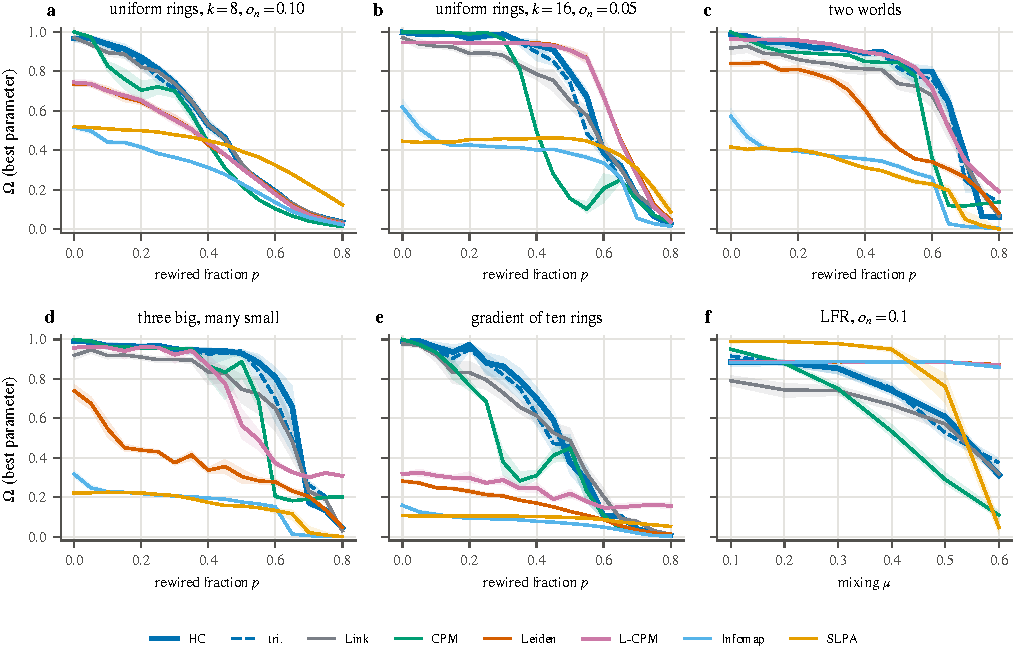
\includegraphics[width=\textwidth]{figures/fig_benchmarks_oracle.pdf}
  \caption{As Fig.~\ref{fig:benchmarks}, with every method at its best parameter on each
  graph (oracle protocol).}
  \label{fig:benchmarksoracle}
\end{figure*}
\clearpage

\begin{table*}[p]
\caption{As Table~\ref{tab:labelfree}, with every method at its best parameter on each test graph (oracle protocol). 95\% bootstrap half-widths of these means over the ten test seeds have median 0.005 and maximum 0.049. Bold: best in row, within 0.005.}
\label{tab:oracle}
\scriptsize\setlength{\tabcolsep}{1.35pt}
\resizebox{\textwidth}{!}{%
\begin{tabular}{llcccc|cc|cccccc|cccccc}
\hline\hline
 & & \multicolumn{4}{c}{HC and ablations} & \multicolumn{2}{c}{relatives} &\multicolumn{6}{c}{partitions} & \multicolumn{6}{c}{overlapping methods} \\
Family & $o_n$ & HC & e-c. & tri. & 2-test & Link & CPM & Leiden & L-CPM & Info. & Walk. & LPA & SBM & SLPA & OSLOM & DEMON & ANGEL & SCAN & SCAN-J \\
\hline
uniform, $k{=}8$ & 0.00 & 0.62$^{-}$ & 0.62 & 0.51 & 0.55 & 0.62 & 0.51 & \textbf{0.68} & \textbf{0.67} & 0.49 & 0.39 & 0.14 & 0.42 & 0.47 & 0.56 & 0.54 & 0.54 & 0.54 & 0.54 \\
 & 0.05 & \textbf{0.57$^{+}$} & \textbf{0.57} & 0.50 & 0.34 & \textbf{0.57} & 0.49 & 0.55 & 0.55 & 0.35 & 0.24 & 0.12 & 0.32 & 0.44 & 0.46 & 0.44 & 0.43 & 0.30 & 0.31 \\
 & 0.10 & \textbf{0.52$^{+}$} & 0.52 & 0.47 & 0.25 & 0.52 & 0.45 & 0.41 & 0.41 & 0.28 & 0.18 & 0.11 & 0.25 & 0.40 & 0.38 & 0.40 & 0.41 & 0.22 & 0.22 \\
\hline
uniform, $k{=}16$ & 0.00 & 0.78$^{-}$ & 0.78 & 0.75 & 0.70 & 0.78 & 0.68 & \textbf{0.86} & 0.85 & 0.47 & 0.65 & 0.14 & 0.51 & 0.44 & 0.73 & 0.64 & 0.67 & 0.65 & 0.59 \\
 & 0.05 & 0.73$^{-}$ & 0.72 & 0.70 & 0.42 & 0.66 & 0.56 & \textbf{0.77} & \textbf{0.77} & 0.35 & 0.47 & 0.11 & 0.38 & 0.41 & 0.66 & 0.51 & 0.63 & 0.34 & 0.36 \\
 & 0.10 & 0.63$^{=}$ & 0.63 & 0.61 & 0.31 & 0.53 & 0.54 & \textbf{0.64} & 0.63 & 0.29 & 0.33 & 0.09 & 0.29 & 0.38 & 0.58 & 0.45 & 0.57 & 0.24 & 0.26 \\
\hline
equal $k$, unequal $s$, $k{=}8$ & 0.00 & 0.58$^{-}$ & 0.57 & 0.46 & 0.51 & 0.57 & 0.46 & \textbf{0.60} & \textbf{0.60} & 0.36 & 0.33 & 0.10 & 0.33 & 0.35 & 0.48 & 0.49 & 0.49 & 0.49 & 0.49 \\
 & 0.05 & \textbf{0.52$^{+}$} & 0.52 & 0.45 & 0.27 & 0.52 & 0.43 & 0.40 & 0.39 & 0.25 & 0.19 & 0.09 & 0.24 & 0.32 & 0.35 & 0.39 & 0.35 & 0.23 & 0.24 \\
 & 0.10 & \textbf{0.46$^{=}$} & 0.45 & 0.41 & 0.19 & \textbf{0.46} & 0.37 & 0.29 & 0.29 & 0.20 & 0.15 & 0.08 & 0.18 & 0.29 & 0.28 & 0.35 & 0.34 & 0.16 & 0.17 \\
\hline
equal $k$, unequal $s$, $k{=}16$ & 0.00 & 0.80$^{-}$ & 0.79 & 0.77 & 0.72 & 0.79 & 0.71 & \textbf{0.87} & \textbf{0.87} & 0.61 & 0.69 & 0.17 & 0.50 & 0.53 & 0.77 & 0.67 & 0.70 & 0.66 & 0.60 \\
 & 0.05 & 0.75$^{-}$ & 0.74 & 0.72 & 0.47 & 0.69 & 0.59 & \textbf{0.79} & 0.78 & 0.51 & 0.56 & 0.14 & 0.42 & 0.50 & 0.71 & 0.55 & 0.66 & 0.39 & 0.39 \\
 & 0.10 & \textbf{0.67$^{+}$} & \textbf{0.67} & 0.65 & 0.35 & 0.59 & 0.57 & 0.66 & 0.65 & 0.44 & 0.44 & 0.12 & 0.36 & 0.46 & 0.65 & 0.49 & 0.62 & 0.28 & 0.29 \\
\hline
equal $s$, unequal $k$ & 0.00 & 0.79$^{-}$ & 0.79 & 0.77 & 0.73 & 0.78 & 0.61 & \textbf{0.82} & \textbf{0.82} & 0.55 & 0.60 & 0.16 & 0.52 & 0.40 & 0.58 & 0.54 & 0.64 & 0.68 & 0.61 \\
 & 0.05 & 0.71$^{-}$ & 0.72 & 0.70 & 0.49 & 0.64 & 0.59 & \textbf{0.72} & \textbf{0.72} & 0.45 & 0.52 & 0.13 & 0.42 & 0.35 & 0.52 & 0.41 & 0.58 & 0.41 & 0.42 \\
 & 0.10 & 0.62$^{-}$ & 0.62 & 0.60 & 0.41 & 0.53 & 0.56 & 0.63 & \textbf{0.65} & 0.39 & 0.46 & 0.11 & 0.35 & 0.31 & 0.47 & 0.34 & 0.49 & 0.32 & 0.35 \\
\hline
two worlds & 0.00 & \textbf{0.84$^{-}$} & \textbf{0.83} & 0.82 & 0.75 & 0.82 & 0.70 & 0.67 & \textbf{0.84} & 0.40 & 0.52 & 0.13 & 0.29 & 0.32 & 0.36 & 0.53 & 0.66 & 0.72 & 0.64 \\
 & 0.05 & 0.78$^{-}$ & 0.78 & 0.77 & 0.59 & 0.71 & 0.68 & 0.56 & \textbf{0.78} & 0.29 & 0.41 & 0.10 & 0.24 & 0.28 & 0.32 & 0.40 & 0.58 & 0.51 & 0.49 \\
 & 0.10 & \textbf{0.72$^{=}$} & \textbf{0.72} & 0.71 & 0.50 & 0.61 & 0.66 & 0.45 & \textbf{0.72} & 0.26 & 0.32 & 0.08 & 0.20 & 0.24 & 0.28 & 0.35 & 0.49 & 0.43 & 0.44 \\
\hline
three big, many small & 0.00 & \textbf{0.84$^{+}$} & \textbf{0.84} & 0.84 & 0.77 & 0.83 & 0.74 & 0.49 & 0.81 & 0.24 & 0.27 & 0.07 & 0.24 & 0.18 & 0.20 & 0.50 & 0.65 & 0.75 & 0.67 \\
 & 0.05 & \textbf{0.80$^{+}$} & \textbf{0.80} & 0.79 & 0.57 & 0.72 & 0.71 & 0.37 & 0.71 & 0.16 & 0.22 & 0.06 & 0.16 & 0.16 & 0.18 & 0.38 & 0.53 & 0.49 & 0.50 \\
 & 0.10 & 0.71$^{+}$ & \textbf{0.72} & 0.69 & 0.48 & 0.61 & 0.67 & 0.26 & 0.48 & 0.14 & 0.17 & 0.05 & 0.13 & 0.13 & 0.16 & 0.33 & 0.45 & 0.42 & 0.44 \\
\hline
gradient & 0.00 & 0.65$^{-}$ & 0.64 & 0.60 & 0.57 & \textbf{0.66} & 0.57 & 0.35 & 0.44 & 0.14 & 0.14 & 0.03 & 0.18 & 0.11 & 0.21 & 0.54 & 0.54 & 0.54 & 0.51 \\
 & 0.05 & \textbf{0.57$^{+}$} & \textbf{0.57} & 0.54 & 0.29 & 0.54 & 0.43 & 0.16 & 0.23 & 0.07 & 0.10 & 0.03 & 0.08 & 0.09 & 0.15 & 0.43 & 0.47 & 0.22 & 0.23 \\
 & 0.10 & \textbf{0.48$^{+}$} & \textbf{0.48} & 0.47 & 0.25 & 0.45 & 0.41 & 0.10 & 0.18 & 0.06 & 0.07 & 0.02 & 0.06 & 0.08 & 0.11 & 0.37 & 0.37 & 0.16 & 0.18 \\
\hline
uniform $k{=}8$, $\alpha{=}1$ & 0.05 & \textbf{0.58$^{+}$} & 0.57 & 0.50 & 0.35 & 0.57 & 0.49 & 0.56 & 0.55 & 0.35 & 0.24 & 0.12 & 0.32 & 0.44 & 0.46 & 0.44 & 0.43 & 0.31 & 0.33 \\
uniform $k{=}8$, $\alpha{=}2$ & 0.05 & \textbf{0.58$^{+}$} & \textbf{0.58} & 0.50 & 0.38 & 0.57 & 0.48 & 0.56 & 0.55 & 0.35 & 0.22 & 0.12 & 0.32 & 0.44 & 0.46 & 0.44 & 0.43 & 0.33 & 0.36 \\
two worlds, $\alpha{=}1$ & 0.05 & 0.78$^{-}$ & 0.78 & 0.76 & 0.56 & 0.70 & 0.67 & 0.61 & \textbf{0.82} & 0.31 & 0.62 & 0.11 & 0.27 & 0.30 & 0.33 & 0.35 & 0.47 & 0.47 & 0.47 \\
two worlds, $\alpha{=}2$ & 0.05 & \textbf{0.79$^{=}$} & \textbf{0.79} & 0.77 & 0.57 & 0.72 & 0.65 & 0.66 & \textbf{0.79} & 0.34 & 0.62 & 0.10 & 0.30 & 0.29 & 0.35 & 0.32 & 0.44 & 0.51 & 0.52 \\
\hline
LFR, $o_n{=}0$ &  & 0.86$^{-}$ & 0.86 & 0.85 & 0.65 & 0.85 & 0.66 & \textbf{1.00} & \textbf{1.00} & \textbf{1.00} & 0.98 & 0.61 & 0.99 & 0.91 & \textbf{1.00} & 0.51 & 0.77 & 0.57 & 0.41 \\
LFR, $o_n{=}0.1$ &  & 0.74$^{-}$ & 0.75 & 0.73 & 0.34 & 0.66 & 0.60 & 0.88 & 0.88 & 0.88 & 0.81 & 0.49 & 0.87 & 0.84 & \textbf{0.97} & 0.46 & 0.73 & 0.33 & 0.25 \\
LFR, $o_n{=}0.3$ &  & 0.50$^{-}$ & 0.53 & 0.51 & 0.16 & 0.42 & 0.48 & 0.69 & 0.69 & 0.66 & 0.49 & 0.32 & 0.57 & 0.71 & \textbf{0.90} & 0.42 & 0.65 & 0.15 & 0.11 \\
LFR, $\langle k\rangle{=}10$ &  & 0.46$^{-}$ & 0.47 & 0.36 & 0.12 & 0.51 & 0.36 & \textbf{0.79} & \textbf{0.79} & 0.71 & 0.61 & 0.36 & 0.63 & 0.53 & 0.78 & 0.27 & 0.31 & 0.15 & 0.13 \\
LFR, $o_m{=}4$ &  & 0.62$^{-}$ & 0.63 & 0.62 & 0.44 & 0.60 & 0.52 & 0.71 & 0.71 & 0.71 & 0.62 & 0.40 & 0.67 & 0.77 & \textbf{0.80} & 0.43 & 0.66 & 0.40 & 0.29 \\
LFR, sizes 50--250 &  & 0.42$^{-}$ & 0.43 & 0.44 & 0.16 & 0.46 & 0.16 & 0.87 & 0.85 & 0.79 & 0.75 & 0.38 & 0.79 & 0.62 & \textbf{0.91} & 0.33 & 0.55 & 0.14 & 0.08 \\
LFR, $C_{\rm LFR}{=}0.3$ &  & 0.39$^{-}$ & 0.40 & 0.39 & 0.24 & 0.31 & 0.42 & \textbf{0.62} & 0.61 & 0.58 & 0.52 & 0.48 & 0.48 & 0.59 & 0.59 & 0.27 & 0.36 & 0.23 & 0.22 \\
LFR, $C_{\rm LFR}{=}0.5$ &  & 0.30$^{-}$ & 0.30 & 0.29 & 0.24 & 0.25 & 0.28 & \textbf{0.38} & \textbf{0.37} & 0.35 & 0.26 & 0.35 & 0.30 & 0.37 & 0.36 & 0.22 & 0.27 & 0.22 & 0.23 \\
\hline\hline
\end{tabular}}
\end{table*}

\begin{table*}[p]
\caption{ONMI (McDaid \emph{et al.}, max normalisation) of the oracle covers of Table~\ref{tab:oracle}; superscripts on HC as in Table~\ref{tab:labelfree}, for ONMI. Bold: best in row, within 0.005.}
\label{tab:onmi-oracle}
\scriptsize\setlength{\tabcolsep}{1.35pt}
\resizebox{\textwidth}{!}{%
\begin{tabular}{llcccc|cc|cccccc|cccccc}
\hline\hline
 & & \multicolumn{4}{c}{HC and ablations} & \multicolumn{2}{c}{relatives} &\multicolumn{6}{c}{partitions} & \multicolumn{6}{c}{overlapping methods} \\
Family & $o_n$ & HC & e-c. & tri. & 2-test & Link & CPM & Leiden & L-CPM & Info. & Walk. & LPA & SBM & SLPA & OSLOM & DEMON & ANGEL & SCAN & SCAN-J \\
\hline
uniform, $k{=}8$ & 0.00 & 0.52$^{-}$ & 0.51 & 0.41 & 0.47 & 0.49 & 0.41 & \textbf{0.61} & \textbf{0.61} & 0.36 & 0.38 & 0.00 & 0.35 & 0.15 & 0.49 & 0.44 & 0.46 & 0.45 & 0.47 \\
 & 0.05 & \textbf{0.47$^{+}$} & 0.46 & 0.39 & 0.20 & 0.42 & 0.39 & 0.46 & 0.45 & 0.18 & 0.22 & 0.00 & 0.23 & 0.12 & 0.36 & 0.28 & 0.28 & 0.16 & 0.19 \\
 & 0.10 & \textbf{0.41$^{+}$} & 0.40 & 0.37 & 0.12 & 0.33 & 0.35 & 0.27 & 0.27 & 0.11 & 0.11 & 0.00 & 0.14 & 0.10 & 0.26 & 0.23 & 0.27 & 0.09 & 0.10 \\
\hline
uniform, $k{=}16$ & 0.00 & 0.71$^{-}$ & 0.71 & 0.67 & 0.65 & 0.51 & 0.59 & \textbf{0.83} & 0.82 & 0.31 & 0.62 & 0.01 & 0.41 & 0.09 & 0.63 & 0.53 & 0.56 & 0.59 & 0.54 \\
 & 0.05 & 0.66$^{-}$ & 0.65 & 0.62 & 0.29 & 0.32 & 0.46 & \textbf{0.71} & \textbf{0.70} & 0.16 & 0.42 & 0.01 & 0.25 & 0.09 & 0.55 & 0.29 & 0.52 & 0.22 & 0.26 \\
 & 0.10 & \textbf{0.56$^{=}$} & \textbf{0.55} & 0.52 & 0.19 & 0.18 & 0.45 & \textbf{0.55} & 0.54 & 0.11 & 0.26 & 0.01 & 0.14 & 0.08 & 0.45 & 0.22 & 0.46 & 0.13 & 0.17 \\
\hline
equal $k$, unequal $s$, $k{=}8$ & 0.00 & 0.49$^{-}$ & 0.48 & 0.38 & 0.44 & 0.46 & 0.38 & \textbf{0.55} & \textbf{0.54} & 0.24 & 0.28 & 0.00 & 0.25 & 0.08 & 0.40 & 0.41 & 0.42 & 0.41 & 0.43 \\
 & 0.05 & \textbf{0.44$^{+}$} & 0.43 & 0.36 & 0.15 & 0.38 & 0.35 & 0.31 & 0.31 & 0.10 & 0.13 & 0.00 & 0.14 & 0.06 & 0.25 & 0.24 & 0.23 & 0.11 & 0.14 \\
 & 0.10 & \textbf{0.36$^{+}$} & 0.36 & 0.32 & 0.08 & 0.30 & 0.30 & 0.17 & 0.17 & 0.06 & 0.06 & 0.00 & 0.08 & 0.05 & 0.16 & 0.20 & 0.21 & 0.05 & 0.08 \\
\hline
equal $k$, unequal $s$, $k{=}16$ & 0.00 & 0.74$^{-}$ & 0.73 & 0.69 & 0.66 & 0.53 & 0.62 & \textbf{0.85} & \textbf{0.85} & 0.52 & 0.71 & 0.07 & 0.43 & 0.26 & 0.71 & 0.57 & 0.60 & 0.61 & 0.55 \\
 & 0.05 & 0.69$^{-}$ & 0.68 & 0.65 & 0.36 & 0.37 & 0.50 & \textbf{0.74} & 0.73 & 0.42 & 0.56 & 0.06 & 0.33 & 0.26 & 0.65 & 0.39 & 0.57 & 0.29 & 0.31 \\
 & 0.10 & \textbf{0.61$^{=}$} & \textbf{0.61} & 0.57 & 0.24 & 0.23 & 0.48 & \textbf{0.61} & 0.60 & 0.36 & 0.44 & 0.05 & 0.27 & 0.24 & 0.59 & 0.30 & 0.52 & 0.18 & 0.21 \\
\hline
equal $s$, unequal $k$ & 0.00 & 0.67$^{-}$ & 0.67 & 0.61 & 0.62 & 0.38 & 0.42 & \textbf{0.76} & 0.70 & 0.38 & 0.56 & 0.05 & 0.49 & 0.14 & 0.45 & 0.40 & 0.46 & 0.58 & 0.52 \\
 & 0.05 & 0.57$^{-}$ & 0.57 & 0.53 & 0.31 & 0.21 & 0.40 & \textbf{0.64} & 0.58 & 0.27 & 0.47 & 0.04 & 0.36 & 0.13 & 0.40 & 0.21 & 0.39 & 0.25 & 0.28 \\
 & 0.10 & 0.45$^{-}$ & 0.44 & 0.42 & 0.24 & 0.12 & 0.36 & \textbf{0.52} & 0.51 & 0.23 & 0.40 & 0.04 & 0.28 & 0.11 & 0.35 & 0.15 & 0.27 & 0.19 & 0.22 \\
\hline
two worlds & 0.00 & 0.62$^{-}$ & 0.60 & 0.54 & 0.56 & 0.34 & 0.32 & 0.54 & \textbf{0.70} & 0.26 & 0.38 & 0.01 & 0.23 & 0.09 & 0.25 & 0.34 & 0.38 & 0.53 & 0.48 \\
 & 0.05 & 0.42$^{-}$ & 0.43 & 0.40 & 0.22 & 0.15 & 0.28 & 0.35 & \textbf{0.57} & 0.14 & 0.25 & 0.01 & 0.18 & 0.06 & 0.20 & 0.15 & 0.28 & 0.19 & 0.21 \\
 & 0.10 & 0.28$^{-}$ & 0.28 & 0.27 & 0.17 & 0.08 & 0.24 & 0.24 & \textbf{0.43} & 0.09 & 0.18 & 0.01 & 0.13 & 0.04 & 0.14 & 0.11 & 0.16 & 0.14 & 0.16 \\
\hline
three big, many small & 0.00 & 0.62$^{-}$ & 0.61 & 0.55 & 0.57 & 0.30 & 0.33 & 0.32 & \textbf{0.69} & 0.15 & 0.19 & 0.00 & 0.18 & 0.06 & 0.16 & 0.29 & 0.36 & 0.54 & 0.48 \\
 & 0.05 & 0.40$^{-}$ & 0.40 & 0.38 & 0.19 & 0.11 & 0.29 & 0.18 & \textbf{0.52} & 0.07 & 0.14 & 0.00 & 0.10 & 0.04 & 0.13 & 0.13 & 0.21 & 0.17 & 0.20 \\
 & 0.10 & 0.26$^{=}$ & \textbf{0.26} & 0.25 & 0.15 & 0.06 & 0.24 & 0.11 & \textbf{0.27} & 0.04 & 0.10 & 0.00 & 0.07 & 0.02 & 0.08 & 0.09 & 0.12 & 0.12 & 0.15 \\
\hline
gradient & 0.00 & \textbf{0.51$^{+}$} & 0.50 & 0.43 & 0.46 & 0.42 & 0.40 & 0.29 & 0.34 & 0.09 & 0.05 & 0.00 & 0.13 & 0.01 & 0.14 & 0.37 & 0.32 & 0.45 & 0.44 \\
 & 0.05 & \textbf{0.38$^{+}$} & \textbf{0.37} & 0.33 & 0.12 & 0.18 & 0.20 & 0.09 & 0.11 & 0.02 & 0.03 & 0.00 & 0.04 & 0.01 & 0.08 & 0.16 & 0.25 & 0.08 & 0.11 \\
 & 0.10 & \textbf{0.23$^{+}$} & \textbf{0.23} & 0.20 & 0.08 & 0.08 & 0.19 & 0.03 & 0.05 & 0.01 & 0.02 & 0.00 & 0.02 & 0.01 & 0.05 & 0.10 & 0.17 & 0.05 & 0.07 \\
\hline
uniform $k{=}8$, $\alpha{=}1$ & 0.05 & \textbf{0.47$^{+}$} & 0.46 & 0.39 & 0.22 & 0.42 & 0.39 & 0.46 & 0.46 & 0.18 & 0.21 & 0.00 & 0.23 & 0.13 & 0.36 & 0.28 & 0.28 & 0.16 & 0.20 \\
uniform $k{=}8$, $\alpha{=}2$ & 0.05 & \textbf{0.48$^{+}$} & 0.47 & 0.39 & 0.25 & 0.41 & 0.38 & 0.46 & 0.46 & 0.18 & 0.20 & 0.00 & 0.23 & 0.12 & 0.36 & 0.28 & 0.28 & 0.19 & 0.23 \\
two worlds, $\alpha{=}1$ & 0.05 & 0.51$^{-}$ & 0.51 & 0.44 & 0.31 & 0.17 & 0.26 & 0.39 & \textbf{0.58} & 0.18 & 0.23 & 0.01 & 0.17 & 0.08 & 0.22 & 0.13 & 0.22 & 0.24 & 0.28 \\
two worlds, $\alpha{=}2$ & 0.05 & \textbf{0.60$^{+}$} & \textbf{0.59} & 0.47 & 0.41 & 0.18 & 0.25 & 0.44 & 0.56 & 0.21 & 0.22 & 0.01 & 0.17 & 0.09 & 0.24 & 0.11 & 0.20 & 0.32 & 0.35 \\
\hline
LFR, $o_n{=}0$ &  & 0.80$^{-}$ & 0.80 & 0.77 & 0.60 & 0.38 & 0.54 & \textbf{1.00} & \textbf{1.00} & \textbf{1.00} & 0.98 & 0.65 & 0.99 & 0.92 & \textbf{1.00} & 0.37 & 0.69 & 0.52 & 0.37 \\
LFR, $o_n{=}0.1$ &  & 0.70$^{-}$ & 0.71 & 0.68 & 0.28 & 0.24 & 0.51 & 0.87 & 0.87 & 0.87 & 0.79 & 0.49 & 0.84 & 0.85 & \textbf{0.96} & 0.28 & 0.64 & 0.29 & 0.22 \\
LFR, $o_n{=}0.3$ &  & 0.49$^{-}$ & 0.51 & 0.49 & 0.12 & 0.12 & 0.45 & 0.69 & 0.69 & 0.67 & 0.55 & 0.28 & 0.58 & 0.70 & \textbf{0.89} & 0.21 & 0.53 & 0.14 & 0.10 \\
LFR, $\langle k\rangle{=}10$ &  & 0.37$^{-}$ & 0.37 & 0.26 & 0.08 & 0.29 & 0.25 & \textbf{0.77} & \textbf{0.77} & 0.68 & 0.57 & 0.36 & 0.62 & 0.37 & \textbf{0.76} & 0.22 & 0.23 & 0.11 & 0.09 \\
LFR, $o_m{=}4$ &  & 0.59$^{-}$ & 0.60 & 0.59 & 0.41 & 0.20 & 0.50 & 0.69 & 0.69 & 0.69 & 0.60 & 0.37 & 0.63 & 0.73 & \textbf{0.78} & 0.35 & 0.59 & 0.39 & 0.30 \\
LFR, sizes 50--250 &  & 0.34$^{-}$ & 0.35 & 0.30 & 0.11 & 0.12 & 0.10 & 0.84 & 0.83 & 0.77 & 0.72 & 0.37 & 0.77 & 0.63 & \textbf{0.90} & 0.15 & 0.42 & 0.10 & 0.06 \\
LFR, $C_{\rm LFR}{=}0.3$ &  & 0.31$^{-}$ & 0.32 & 0.31 & 0.17 & 0.08 & 0.31 & \textbf{0.57} & 0.56 & 0.54 & 0.48 & 0.45 & 0.39 & 0.51 & 0.54 & 0.13 & 0.20 & 0.17 & 0.16 \\
LFR, $C_{\rm LFR}{=}0.5$ &  & 0.19$^{-}$ & 0.19 & 0.18 & 0.13 & 0.04 & 0.13 & \textbf{0.30} & 0.28 & 0.25 & 0.18 & 0.26 & 0.17 & 0.22 & 0.26 & 0.08 & 0.08 & 0.12 & 0.13 \\
\hline\hline
\end{tabular}}
\end{table*}

\begin{table*}[p]
\caption{ONMI (McDaid \emph{et al.}, max normalisation) of the label-free covers of Table~\ref{tab:labelfree}; superscripts on HC as in Table~\ref{tab:labelfree}, for ONMI. Bold: best in row, within 0.005.}
\label{tab:onmi-label-free}
\scriptsize\setlength{\tabcolsep}{1.35pt}
\resizebox{\textwidth}{!}{%
\begin{tabular}{llcccc|cc|cccccc|cccccc}
\hline\hline
 & & \multicolumn{4}{c}{HC and ablations} & \multicolumn{2}{c}{relatives} &\multicolumn{6}{c}{partitions} & \multicolumn{6}{c}{overlapping methods} \\
Family & $o_n$ & HC & e-c. & tri. & 2-test & Link & CPM & Leiden & L-CPM & Info. & Walk. & LPA & SBM & SLPA & OSLOM & DEMON & ANGEL & SCAN & SCAN-J \\
\hline
uniform, $k{=}8$ & 0.00 & 0.52$^{-}$ & 0.51 & 0.41 & 0.46 & 0.49 & 0.41 & \textbf{0.57} & \textbf{0.57} & 0.36 & 0.38 & 0.00 & 0.31 & 0.07 & 0.47 & 0.44 & 0.46 & 0.45 & 0.47 \\
 & 0.05 & \textbf{0.47$^{+}$} & 0.46 & 0.39 & 0.20 & 0.43 & 0.39 & 0.36 & 0.35 & 0.17 & 0.22 & 0.00 & 0.18 & 0.06 & 0.35 & 0.28 & 0.29 & 0.17 & 0.19 \\
 & 0.10 & \textbf{0.41$^{+}$} & 0.41 & 0.36 & 0.12 & 0.36 & 0.35 & 0.20 & 0.19 & 0.09 & 0.11 & 0.00 & 0.10 & 0.04 & 0.25 & 0.22 & 0.27 & 0.09 & 0.11 \\
\hline
uniform, $k{=}16$ & 0.00 & 0.72$^{-}$ & 0.71 & 0.67 & 0.65 & 0.52 & 0.60 & \textbf{0.82} & 0.82 & 0.31 & 0.62 & 0.01 & 0.41 & 0.05 & 0.61 & 0.53 & 0.56 & 0.59 & 0.54 \\
 & 0.05 & 0.66$^{-}$ & 0.65 & 0.62 & 0.30 & 0.37 & 0.46 & \textbf{0.70} & \textbf{0.69} & 0.17 & 0.42 & 0.01 & 0.24 & 0.05 & 0.52 & 0.33 & 0.53 & 0.23 & 0.26 \\
 & 0.10 & \textbf{0.56$^{+}$} & \textbf{0.55} & 0.52 & 0.19 & 0.24 & 0.45 & 0.53 & 0.52 & 0.11 & 0.26 & 0.01 & 0.14 & 0.05 & 0.41 & 0.25 & 0.47 & 0.14 & 0.17 \\
\hline
equal $k$, unequal $s$, $k{=}8$ & 0.00 & 0.49$^{-}$ & 0.48 & 0.38 & 0.44 & 0.46 & 0.38 & \textbf{0.52} & 0.51 & 0.24 & 0.28 & 0.00 & 0.25 & 0.03 & 0.39 & 0.40 & 0.42 & 0.42 & 0.44 \\
 & 0.05 & \textbf{0.44$^{+}$} & 0.43 & 0.36 & 0.16 & 0.40 & 0.35 & 0.27 & 0.27 & 0.10 & 0.13 & 0.00 & 0.13 & 0.03 & 0.24 & 0.22 & 0.23 & 0.12 & 0.14 \\
 & 0.10 & \textbf{0.37$^{+}$} & 0.35 & 0.32 & 0.09 & 0.33 & 0.30 & 0.13 & 0.13 & 0.05 & 0.06 & 0.00 & 0.06 & 0.02 & 0.15 & 0.16 & 0.21 & 0.06 & 0.08 \\
\hline
equal $k$, unequal $s$, $k{=}16$ & 0.00 & 0.74$^{-}$ & 0.73 & 0.69 & 0.67 & 0.54 & 0.63 & \textbf{0.82} & \textbf{0.82} & 0.52 & 0.71 & 0.07 & 0.41 & 0.23 & 0.70 & 0.56 & 0.60 & 0.61 & 0.55 \\
 & 0.05 & \textbf{0.68$^{+}$} & \textbf{0.68} & 0.64 & 0.36 & 0.40 & 0.50 & 0.67 & 0.67 & 0.42 & 0.56 & 0.06 & 0.30 & 0.23 & 0.64 & 0.43 & 0.57 & 0.31 & 0.30 \\
 & 0.10 & \textbf{0.60$^{+}$} & \textbf{0.60} & 0.57 & 0.23 & 0.29 & 0.48 & 0.51 & 0.50 & 0.36 & 0.44 & 0.05 & 0.23 & 0.21 & 0.58 & 0.37 & 0.52 & 0.19 & 0.21 \\
\hline
equal $s$, unequal $k$ & 0.00 & 0.67$^{-}$ & 0.67 & 0.61 & 0.63 & 0.36 & 0.40 & \textbf{0.76} & 0.71 & 0.39 & 0.56 & 0.05 & 0.50 & 0.14 & 0.46 & 0.46 & 0.46 & 0.59 & 0.52 \\
 & 0.05 & 0.55$^{-}$ & 0.54 & 0.51 & 0.31 & 0.23 & 0.40 & \textbf{0.61} & 0.58 & 0.28 & 0.47 & 0.04 & 0.36 & 0.13 & 0.39 & 0.31 & 0.40 & 0.26 & 0.28 \\
 & 0.10 & 0.44$^{-}$ & 0.45 & 0.42 & 0.24 & 0.13 & 0.37 & 0.49 & \textbf{0.50} & 0.23 & 0.40 & 0.04 & 0.27 & 0.12 & 0.35 & 0.25 & 0.35 & 0.19 & 0.22 \\
\hline
two worlds & 0.00 & 0.62$^{-}$ & 0.61 & 0.54 & 0.56 & 0.29 & 0.31 & 0.48 & \textbf{0.67} & 0.26 & 0.38 & 0.01 & 0.23 & 0.05 & 0.16 & 0.39 & 0.39 & 0.53 & 0.48 \\
 & 0.05 & \textbf{0.45$^{=}$} & \textbf{0.45} & 0.41 & 0.22 & 0.17 & 0.30 & 0.29 & 0.45 & 0.14 & 0.25 & 0.01 & 0.18 & 0.04 & 0.09 & 0.26 & 0.34 & 0.19 & 0.21 \\
 & 0.10 & \textbf{0.28$^{+}$} & \textbf{0.29} & 0.27 & 0.17 & 0.09 & 0.25 & 0.19 & 0.27 & 0.09 & 0.18 & 0.01 & 0.13 & 0.03 & 0.05 & 0.20 & 0.26 & 0.14 & 0.16 \\
\hline
three big, many small & 0.00 & \textbf{0.63$^{+}$} & 0.62 & 0.55 & 0.57 & 0.25 & 0.32 & 0.32 & 0.37 & 0.14 & 0.19 & 0.00 & 0.15 & 0.03 & 0.11 & 0.33 & 0.38 & 0.54 & 0.48 \\
 & 0.05 & 0.39$^{+}$ & \textbf{0.40} & 0.37 & 0.17 & 0.13 & 0.28 & 0.19 & 0.27 & 0.08 & 0.14 & 0.00 & 0.09 & 0.02 & 0.06 & 0.13 & 0.26 & 0.15 & 0.17 \\
 & 0.10 & \textbf{0.25$^{+}$} & \textbf{0.24} & 0.23 & 0.12 & 0.06 & 0.22 & 0.11 & 0.18 & 0.04 & 0.10 & 0.00 & 0.06 & 0.01 & 0.03 & 0.09 & 0.15 & 0.11 & 0.14 \\
\hline
gradient & 0.00 & 0.27$^{-}$ & 0.24 & 0.25 & 0.23 & \textbf{0.40} & 0.38 & 0.20 & 0.16 & 0.05 & 0.05 & 0.00 & 0.10 & 0.01 & 0.13 & 0.35 & 0.29 & 0.31 & 0.26 \\
 & 0.05 & 0.15$^{-}$ & 0.14 & 0.11 & 0.07 & 0.19 & 0.18 & 0.08 & 0.09 & 0.02 & 0.03 & 0.00 & 0.03 & 0.01 & 0.07 & 0.09 & \textbf{0.23} & 0.07 & 0.08 \\
 & 0.10 & 0.07$^{-}$ & 0.07 & 0.06 & 0.03 & 0.09 & \textbf{0.16} & 0.03 & 0.04 & 0.01 & 0.02 & 0.00 & 0.02 & 0.01 & 0.04 & 0.05 & 0.15 & 0.04 & 0.05 \\
\hline
uniform $k{=}8$, $\alpha{=}1$ & 0.05 & \textbf{0.47$^{+}$} & 0.46 & 0.39 & 0.22 & 0.43 & 0.39 & 0.36 & 0.36 & 0.18 & 0.21 & 0.00 & 0.19 & 0.05 & 0.35 & 0.28 & 0.28 & 0.18 & 0.21 \\
uniform $k{=}8$, $\alpha{=}2$ & 0.05 & \textbf{0.48$^{+}$} & 0.47 & 0.39 & 0.25 & 0.43 & 0.38 & 0.36 & 0.36 & 0.17 & 0.20 & 0.00 & 0.18 & 0.05 & 0.35 & 0.28 & 0.29 & 0.21 & 0.23 \\
two worlds, $\alpha{=}1$ & 0.05 & \textbf{0.52$^{+}$} & \textbf{0.51} & 0.43 & 0.31 & 0.19 & 0.28 & 0.33 & 0.44 & 0.17 & 0.23 & 0.01 & 0.16 & 0.05 & 0.11 & 0.24 & 0.30 & 0.24 & 0.28 \\
two worlds, $\alpha{=}2$ & 0.05 & \textbf{0.59$^{+}$} & \textbf{0.59} & 0.46 & 0.43 & 0.19 & 0.28 & 0.37 & 0.44 & 0.19 & 0.22 & 0.01 & 0.16 & 0.06 & 0.14 & 0.22 & 0.27 & 0.33 & 0.36 \\
\hline
LFR, $o_n{=}0$ &  & 0.80$^{-}$ & 0.80 & 0.77 & 0.57 & 0.38 & 0.54 & 0.97 & 0.97 & \textbf{1.00} & 0.98 & 0.65 & 0.99 & 0.92 & \textbf{0.99} & 0.47 & 0.70 & 0.49 & 0.36 \\
LFR, $o_n{=}0.1$ &  & 0.66$^{-}$ & 0.69 & 0.67 & 0.26 & 0.24 & 0.51 & 0.68 & 0.68 & 0.86 & 0.79 & 0.49 & 0.84 & 0.79 & \textbf{0.92} & 0.41 & 0.66 & 0.28 & 0.22 \\
LFR, $o_n{=}0.3$ &  & 0.44$^{-}$ & 0.48 & 0.44 & 0.10 & 0.12 & 0.45 & 0.35 & 0.35 & 0.64 & 0.55 & 0.28 & 0.38 & 0.59 & \textbf{0.83} & 0.38 & 0.57 & 0.13 & 0.10 \\
LFR, $\langle k\rangle{=}10$ &  & 0.36$^{-}$ & 0.37 & 0.26 & 0.07 & 0.30 & 0.25 & 0.58 & 0.60 & 0.67 & 0.57 & 0.36 & 0.62 & 0.40 & \textbf{0.74} & 0.23 & 0.19 & 0.10 & 0.09 \\
LFR, $o_m{=}4$ &  & 0.58$^{-}$ & 0.60 & 0.58 & 0.38 & 0.19 & 0.50 & 0.47 & 0.47 & 0.68 & 0.60 & 0.37 & 0.63 & 0.64 & \textbf{0.71} & 0.42 & 0.61 & 0.37 & 0.31 \\
LFR, sizes 50--250 &  & 0.35$^{-}$ & 0.34 & 0.30 & 0.10 & 0.13 & 0.10 & 0.84 & 0.82 & 0.77 & 0.72 & 0.37 & 0.77 & 0.59 & \textbf{0.88} & 0.17 & 0.42 & 0.10 & 0.06 \\
LFR, $C_{\rm LFR}{=}0.3$ &  & 0.28$^{-}$ & 0.28 & 0.28 & 0.15 & 0.08 & 0.29 & 0.35 & 0.35 & 0.47 & 0.48 & 0.45 & 0.22 & \textbf{0.50} & 0.46 & 0.19 & 0.23 & 0.16 & 0.16 \\
LFR, $C_{\rm LFR}{=}0.5$ &  & 0.16$^{-}$ & 0.16 & 0.15 & 0.11 & 0.04 & 0.11 & 0.12 & 0.12 & 0.17 & 0.18 & \textbf{0.26} & 0.11 & 0.24 & 0.23 & 0.10 & 0.10 & 0.10 & 0.12 \\
\hline\hline
\end{tabular}}
\end{table*}

\begin{table*}[p]
\caption{Per-community recovery of the true communities no larger than the median size, oracle covers, on the unequal-ring families (equal $s$ with unequal $k$ has no community larger than the median). Numbers of rings no larger than the median size: $20$, $20$, $20$, $20$, $16$, $5$ (families in order). Bold: best in row, within 0.005.}
\label{tab:recsmall}
\scriptsize\setlength{\tabcolsep}{1.35pt}
\resizebox{\textwidth}{!}{%
\begin{tabular}{llcccc|cc|cccccc|cccccc}
\hline\hline
 & & \multicolumn{4}{c}{HC and ablations} & \multicolumn{2}{c}{relatives} &\multicolumn{6}{c}{partitions} & \multicolumn{6}{c}{overlapping methods} \\
Family & $o_n$ & HC & e-c. & tri. & 2-test & Link & CPM & Leiden & L-CPM & Info. & Walk. & LPA & SBM & SLPA & OSLOM & DEMON & ANGEL & SCAN & SCAN-J \\
\hline
equal $k$, unequal $s$, $k{=}8$ & 0.00 & 0.62 & 0.62 & 0.52 & 0.57 & 0.62 & 0.52 & \textbf{0.68} & \textbf{0.67} & 0.47 & 0.49 & 0.15 & 0.32 & 0.39 & 0.55 & 0.57 & 0.55 & 0.55 & 0.55 \\
 & 0.05 & \textbf{0.58} & \textbf{0.58} & 0.51 & 0.35 & 0.57 & 0.50 & 0.53 & 0.53 & 0.34 & 0.35 & 0.14 & 0.28 & 0.37 & 0.46 & 0.48 & 0.42 & 0.32 & 0.33 \\
 & 0.10 & \textbf{0.52} & 0.51 & 0.47 & 0.28 & \textbf{0.52} & 0.45 & 0.41 & 0.41 & 0.29 & 0.28 & 0.13 & 0.24 & 0.35 & 0.38 & 0.44 & 0.41 & 0.26 & 0.26 \\
\hline
equal $k$, unequal $s$, $k{=}16$ & 0.00 & 0.82 & 0.82 & 0.80 & 0.76 & 0.82 & 0.75 & \textbf{0.91} & 0.90 & 0.78 & 0.83 & 0.23 & 0.53 & 0.59 & 0.84 & 0.77 & 0.74 & 0.71 & 0.65 \\
 & 0.05 & 0.78 & 0.78 & 0.76 & 0.54 & 0.74 & 0.66 & \textbf{0.83} & 0.81 & 0.74 & 0.73 & 0.19 & 0.46 & 0.57 & 0.80 & 0.72 & 0.71 & 0.48 & 0.48 \\
 & 0.10 & 0.72 & 0.72 & 0.69 & 0.44 & 0.65 & 0.63 & 0.73 & 0.72 & 0.66 & 0.66 & 0.17 & 0.43 & 0.54 & \textbf{0.77} & 0.67 & 0.67 & 0.38 & 0.39 \\
\hline
equal $s$, unequal $k$ & 0.00 & 0.77 & 0.77 & 0.73 & 0.72 & 0.75 & 0.57 & \textbf{0.80} & 0.78 & 0.50 & 0.65 & 0.17 & 0.54 & 0.33 & 0.52 & 0.60 & 0.61 & 0.68 & 0.62 \\
 & 0.05 & 0.68 & 0.69 & 0.66 & 0.47 & 0.61 & 0.55 & \textbf{0.70} & 0.68 & 0.40 & 0.56 & 0.15 & 0.44 & 0.30 & 0.47 & 0.48 & 0.55 & 0.41 & 0.42 \\
 & 0.10 & 0.58 & 0.58 & 0.56 & 0.40 & 0.52 & 0.51 & \textbf{0.61} & \textbf{0.61} & 0.35 & 0.51 & 0.14 & 0.38 & 0.28 & 0.43 & 0.42 & 0.47 & 0.33 & 0.35 \\
\hline
two worlds & 0.00 & 0.61 & 0.60 & 0.52 & 0.56 & 0.56 & 0.27 & 0.47 & \textbf{0.68} & 0.39 & 0.38 & 0.13 & 0.18 & 0.30 & 0.55 & 0.45 & 0.41 & 0.54 & 0.50 \\
 & 0.05 & 0.38 & 0.39 & 0.35 & 0.20 & 0.30 & 0.20 & 0.26 & \textbf{0.54} & 0.30 & 0.28 & 0.11 & 0.15 & 0.26 & 0.44 & 0.31 & 0.33 & 0.20 & 0.22 \\
 & 0.10 & 0.21 & 0.21 & 0.19 & 0.16 & 0.21 & 0.14 & 0.15 & \textbf{0.38} & 0.25 & 0.23 & 0.09 & 0.13 & 0.23 & 0.33 & 0.27 & 0.24 & 0.15 & 0.18 \\
\hline
three big, many small & 0.00 & 0.60 & 0.59 & 0.53 & 0.57 & 0.56 & 0.26 & 0.22 & \textbf{0.69} & 0.35 & 0.32 & 0.12 & 0.10 & 0.30 & 0.46 & 0.42 & 0.38 & 0.53 & 0.50 \\
 & 0.05 & 0.33 & 0.34 & 0.31 & 0.19 & 0.27 & 0.20 & 0.11 & \textbf{0.53} & 0.29 & 0.25 & 0.11 & 0.14 & 0.26 & 0.37 & 0.30 & 0.28 & 0.19 & 0.22 \\
 & 0.10 & 0.17 & 0.17 & 0.16 & 0.16 & 0.19 & 0.14 & 0.14 & \textbf{0.37} & 0.24 & 0.21 & 0.09 & 0.13 & 0.22 & 0.26 & 0.27 & 0.21 & 0.15 & 0.17 \\
\hline
gradient & 0.00 & \textbf{0.59} & \textbf{0.59} & 0.50 & 0.56 & 0.57 & 0.49 & 0.32 & 0.52 & 0.35 & 0.37 & 0.13 & 0.19 & 0.36 & 0.33 & 0.49 & 0.42 & 0.53 & 0.52 \\
 & 0.05 & \textbf{0.48} & \textbf{0.48} & 0.42 & 0.29 & 0.41 & 0.32 & 0.27 & 0.29 & 0.28 & 0.29 & 0.12 & 0.18 & 0.34 & 0.26 & 0.41 & 0.37 & 0.24 & 0.27 \\
 & 0.10 & 0.35 & 0.35 & 0.31 & 0.22 & 0.32 & 0.30 & 0.22 & 0.20 & 0.25 & 0.24 & 0.11 & 0.16 & 0.30 & 0.20 & \textbf{0.36} & 0.31 & 0.19 & 0.20 \\
\hline\hline
\end{tabular}}
\end{table*}

\begin{table*}[p]
\caption{Per-community recovery of the true communities larger than the median size, oracle covers, on the unequal-ring families (equal $s$ with unequal $k$ has no community larger than the median). Numbers of rings larger than the median size: $10$, $10$, $5$, $3$, $5$ (families in order). Bold: best in row, within 0.005.}
\label{tab:reclarge}
\scriptsize\setlength{\tabcolsep}{1.35pt}
\resizebox{\textwidth}{!}{%
\begin{tabular}{llcccc|cc|cccccc|cccccc}
\hline\hline
 & & \multicolumn{4}{c}{HC and ablations} & \multicolumn{2}{c}{relatives} &\multicolumn{6}{c}{partitions} & \multicolumn{6}{c}{overlapping methods} \\
Family & $o_n$ & HC & e-c. & tri. & 2-test & Link & CPM & Leiden & L-CPM & Info. & Walk. & LPA & SBM & SLPA & OSLOM & DEMON & ANGEL & SCAN & SCAN-J \\
\hline
equal $k$, unequal $s$, $k{=}8$ & 0.00 & 0.56 & 0.55 & 0.44 & 0.50 & 0.55 & 0.44 & \textbf{0.57} & \textbf{0.57} & 0.28 & 0.32 & 0.11 & 0.32 & 0.22 & 0.46 & 0.49 & 0.47 & 0.48 & 0.49 \\
 & 0.05 & \textbf{0.50} & 0.49 & 0.43 & 0.25 & 0.49 & 0.41 & 0.32 & 0.31 & 0.19 & 0.20 & 0.10 & 0.21 & 0.21 & 0.31 & 0.40 & 0.31 & 0.22 & 0.24 \\
 & 0.10 & \textbf{0.43} & 0.42 & 0.38 & 0.20 & 0.42 & 0.36 & 0.24 & 0.23 & 0.17 & 0.17 & 0.10 & 0.16 & 0.20 & 0.24 & 0.36 & 0.29 & 0.17 & 0.18 \\
\hline
equal $k$, unequal $s$, $k{=}16$ & 0.00 & 0.79 & 0.79 & 0.76 & 0.72 & 0.79 & 0.70 & \textbf{0.85} & \textbf{0.86} & 0.43 & 0.69 & 0.15 & 0.45 & 0.33 & 0.71 & 0.71 & 0.67 & 0.67 & 0.61 \\
 & 0.05 & 0.74 & 0.74 & 0.71 & 0.46 & 0.69 & 0.58 & \textbf{0.76} & \textbf{0.76} & 0.30 & 0.53 & 0.14 & 0.36 & 0.32 & 0.64 & 0.63 & 0.64 & 0.39 & 0.40 \\
 & 0.10 & \textbf{0.66} & \textbf{0.66} & 0.64 & 0.35 & 0.58 & 0.56 & 0.62 & 0.62 & 0.27 & 0.40 & 0.13 & 0.30 & 0.31 & 0.57 & 0.56 & 0.59 & 0.30 & 0.31 \\
\hline
two worlds & 0.00 & \textbf{0.88} & \textbf{0.88} & 0.87 & 0.81 & 0.87 & 0.77 & 0.73 & 0.87 & 0.38 & 0.62 & 0.17 & 0.48 & 0.27 & 0.24 & 0.65 & 0.71 & 0.78 & 0.70 \\
 & 0.05 & \textbf{0.85} & \textbf{0.85} & 0.84 & 0.67 & 0.81 & 0.76 & 0.68 & 0.83 & 0.26 & 0.51 & 0.16 & 0.41 & 0.25 & 0.24 & 0.55 & 0.64 & 0.58 & 0.56 \\
 & 0.10 & \textbf{0.81} & \textbf{0.81} & 0.80 & 0.58 & 0.72 & 0.74 & 0.60 & 0.79 & 0.24 & 0.42 & 0.16 & 0.37 & 0.24 & 0.24 & 0.51 & 0.55 & 0.50 & 0.51 \\
\hline
three big, many small & 0.00 & \textbf{0.87} & \textbf{0.87} & 0.86 & 0.80 & 0.86 & 0.78 & 0.58 & 0.82 & 0.23 & 0.28 & 0.18 & 0.44 & 0.17 & 0.16 & 0.63 & 0.70 & 0.78 & 0.71 \\
 & 0.05 & \textbf{0.84} & \textbf{0.84} & 0.83 & 0.60 & 0.77 & 0.76 & 0.47 & 0.72 & 0.15 & 0.26 & 0.19 & 0.30 & 0.17 & 0.16 & 0.55 & 0.58 & 0.52 & 0.54 \\
 & 0.10 & 0.77 & \textbf{0.77} & 0.74 & 0.53 & 0.68 & 0.72 & 0.31 & 0.47 & 0.13 & 0.23 & 0.20 & 0.26 & 0.17 & 0.16 & 0.47 & 0.51 & 0.44 & 0.48 \\
\hline
gradient & 0.00 & \textbf{0.60} & 0.59 & 0.52 & 0.54 & 0.59 & 0.50 & 0.40 & 0.44 & 0.17 & 0.15 & 0.12 & 0.27 & 0.11 & 0.29 & 0.50 & 0.44 & 0.51 & 0.49 \\
 & 0.05 & \textbf{0.49} & \textbf{0.49} & 0.43 & 0.25 & 0.42 & 0.32 & 0.20 & 0.26 & 0.10 & 0.13 & 0.13 & 0.20 & 0.11 & 0.21 & 0.37 & 0.38 & 0.20 & 0.21 \\
 & 0.10 & \textbf{0.37} & \textbf{0.36} & 0.33 & 0.22 & 0.33 & 0.31 & 0.15 & 0.22 & 0.09 & 0.12 & 0.14 & 0.17 & 0.10 & 0.17 & 0.31 & 0.31 & 0.18 & 0.17 \\
\hline\hline
\end{tabular}}
\end{table*}

\begin{table*}[p]
\caption{Coverage (fraction of nodes in at least one community) of the label-free covers.}
\label{tab:S-coverage-label-free}
\scriptsize\setlength{\tabcolsep}{1.35pt}
\resizebox{\textwidth}{!}{%
\begin{tabular}{llcccc|cc|cccccc|cccccc}
\hline\hline
 & & \multicolumn{4}{c}{HC and ablations} & \multicolumn{2}{c}{relatives} &\multicolumn{6}{c}{partitions} & \multicolumn{6}{c}{overlapping methods} \\
Family & $o_n$ & HC & e-c. & tri. & 2-test & Link & CPM & Leiden & L-CPM & Info. & Walk. & LPA & SBM & SLPA & OSLOM & DEMON & ANGEL & SCAN & SCAN-J \\
\hline
uniform, $k{=}8$ & 0.00 & 0.96 & 0.97 & 0.79 & 0.82 & 0.97 & 0.79 & 1.00 & 1.00 & 1.00 & 1.00 & 1.00 & 1.00 & 0.99 & 1.00 & 0.71 & 0.71 & 0.80 & 0.74 \\
 & 0.05 & 0.96 & 0.97 & 0.80 & 0.77 & 0.97 & 0.80 & 1.00 & 1.00 & 1.00 & 1.00 & 1.00 & 1.00 & 0.99 & 1.00 & 0.72 & 0.71 & 0.73 & 0.68 \\
 & 0.10 & 0.96 & 0.96 & 0.81 & 0.75 & 0.97 & 0.81 & 1.00 & 1.00 & 1.00 & 1.00 & 1.00 & 1.00 & 0.99 & 1.00 & 0.73 & 0.72 & 0.68 & 0.63 \\
\hline
uniform, $k{=}16$ & 0.00 & 0.95 & 0.95 & 0.96 & 0.86 & 0.97 & 0.97 & 1.00 & 1.00 & 1.00 & 1.00 & 1.00 & 1.00 & 1.00 & 1.00 & 0.93 & 0.91 & 0.84 & 0.79 \\
 & 0.05 & 0.94 & 0.94 & 0.95 & 0.78 & 0.97 & 0.93 & 1.00 & 1.00 & 1.00 & 1.00 & 1.00 & 1.00 & 0.99 & 1.00 & 0.93 & 0.92 & 0.75 & 0.71 \\
 & 0.10 & 0.92 & 0.92 & 0.94 & 0.75 & 0.97 & 0.92 & 1.00 & 1.00 & 1.00 & 1.00 & 1.00 & 1.00 & 0.99 & 1.00 & 0.94 & 0.92 & 0.69 & 0.67 \\
\hline
equal $k$, unequal $s$, $k{=}8$ & 0.00 & 0.96 & 0.97 & 0.79 & 0.82 & 0.97 & 0.79 & 1.00 & 1.00 & 1.00 & 1.00 & 1.00 & 1.00 & 0.99 & 1.00 & 0.71 & 0.71 & 0.80 & 0.74 \\
 & 0.05 & 0.96 & 0.96 & 0.80 & 0.76 & 0.97 & 0.80 & 1.00 & 1.00 & 1.00 & 1.00 & 1.00 & 1.00 & 0.99 & 1.00 & 0.72 & 0.71 & 0.73 & 0.68 \\
 & 0.10 & 0.96 & 0.96 & 0.81 & 0.74 & 0.97 & 0.81 & 1.00 & 1.00 & 1.00 & 1.00 & 1.00 & 1.00 & 0.99 & 1.00 & 0.73 & 0.72 & 0.68 & 0.63 \\
\hline
equal $k$, unequal $s$, $k{=}16$ & 0.00 & 0.95 & 0.95 & 0.96 & 0.86 & 0.97 & 0.97 & 1.00 & 1.00 & 1.00 & 1.00 & 1.00 & 1.00 & 0.99 & 1.00 & 0.93 & 0.91 & 0.84 & 0.80 \\
 & 0.05 & 0.94 & 0.94 & 0.95 & 0.80 & 0.97 & 0.95 & 1.00 & 1.00 & 1.00 & 1.00 & 1.00 & 1.00 & 0.99 & 1.00 & 0.93 & 0.92 & 0.76 & 0.72 \\
 & 0.10 & 0.92 & 0.92 & 0.95 & 0.75 & 0.97 & 0.91 & 1.00 & 1.00 & 1.00 & 1.00 & 1.00 & 1.00 & 0.99 & 1.00 & 0.94 & 0.92 & 0.70 & 0.67 \\
\hline
equal $s$, unequal $k$ & 0.00 & 0.93 & 0.93 & 0.94 & 0.86 & 0.96 & 0.85 & 1.00 & 1.00 & 1.00 & 1.00 & 1.00 & 1.00 & 0.99 & 1.00 & 0.93 & 0.91 & 0.83 & 0.83 \\
 & 0.05 & 0.92 & 0.92 & 0.93 & 0.77 & 0.95 & 0.84 & 1.00 & 1.00 & 1.00 & 1.00 & 1.00 & 1.00 & 0.99 & 1.00 & 0.94 & 0.92 & 0.71 & 0.72 \\
 & 0.10 & 0.88 & 0.90 & 0.90 & 0.71 & 0.94 & 0.82 & 1.00 & 1.00 & 1.00 & 1.00 & 1.00 & 1.00 & 0.99 & 1.00 & 0.95 & 0.93 & 0.64 & 0.67 \\
\hline
two worlds & 0.00 & 0.93 & 0.93 & 0.90 & 0.85 & 0.92 & 0.75 & 1.00 & 1.00 & 1.00 & 1.00 & 1.00 & 1.00 & 0.99 & 1.00 & 0.90 & 0.87 & 0.80 & 0.79 \\
 & 0.05 & 0.89 & 0.89 & 0.87 & 0.67 & 0.92 & 0.74 & 1.00 & 1.00 & 1.00 & 1.00 & 1.00 & 1.00 & 0.99 & 1.00 & 0.91 & 0.88 & 0.63 & 0.66 \\
 & 0.10 & 0.81 & 0.82 & 0.81 & 0.62 & 0.91 & 0.70 & 1.00 & 1.00 & 1.00 & 1.00 & 1.00 & 1.00 & 0.99 & 1.00 & 0.93 & 0.89 & 0.57 & 0.63 \\
\hline
three big, many small & 0.00 & 0.92 & 0.92 & 0.90 & 0.85 & 0.94 & 0.79 & 1.00 & 1.00 & 1.00 & 1.00 & 1.00 & 1.00 & 0.99 & 1.00 & 0.92 & 0.90 & 0.81 & 0.78 \\
 & 0.05 & 0.84 & 0.86 & 0.85 & 0.64 & 0.93 & 0.75 & 1.00 & 1.00 & 1.00 & 1.00 & 1.00 & 1.00 & 0.99 & 1.00 & 0.94 & 0.91 & 0.60 & 0.63 \\
 & 0.10 & 0.77 & 0.78 & 0.77 & 0.60 & 0.91 & 0.68 & 1.00 & 1.00 & 1.00 & 1.00 & 1.00 & 1.00 & 0.99 & 1.00 & 0.95 & 0.91 & 0.55 & 0.64 \\
\hline
gradient & 0.00 & 0.93 & 0.93 & 0.87 & 0.82 & 0.95 & 0.88 & 1.00 & 1.00 & 1.00 & 1.00 & 1.00 & 1.00 & 0.99 & 1.00 & 0.83 & 0.82 & 0.80 & 0.74 \\
 & 0.05 & 0.91 & 0.92 & 0.86 & 0.76 & 0.95 & 0.86 & 1.00 & 1.00 & 1.00 & 1.00 & 1.00 & 1.00 & 0.99 & 1.00 & 0.84 & 0.82 & 0.72 & 0.70 \\
 & 0.10 & 0.90 & 0.91 & 0.86 & 0.72 & 0.95 & 0.84 & 1.00 & 1.00 & 1.00 & 1.00 & 1.00 & 1.00 & 0.99 & 1.00 & 0.85 & 0.83 & 0.71 & 0.66 \\
\hline
uniform $k{=}8$, $\alpha{=}1$ & 0.05 & 0.97 & 0.97 & 0.80 & 0.78 & 0.98 & 0.81 & 1.00 & 1.00 & 1.00 & 1.00 & 1.00 & 1.00 & 0.99 & 1.00 & 0.72 & 0.71 & 0.75 & 0.68 \\
uniform $k{=}8$, $\alpha{=}2$ & 0.05 & 0.97 & 0.97 & 0.81 & 0.80 & 0.98 & 0.81 & 1.00 & 1.00 & 1.00 & 1.00 & 1.00 & 1.00 & 0.99 & 1.00 & 0.73 & 0.72 & 0.78 & 0.71 \\
two worlds, $\alpha{=}1$ & 0.05 & 0.91 & 0.92 & 0.86 & 0.82 & 0.94 & 0.71 & 1.00 & 1.00 & 1.00 & 1.00 & 1.00 & 1.00 & 0.99 & 1.00 & 0.89 & 0.87 & 0.75 & 0.74 \\
two worlds, $\alpha{=}2$ & 0.05 & 0.93 & 0.93 & 0.86 & 0.88 & 0.95 & 0.71 & 1.00 & 1.00 & 1.00 & 1.00 & 1.00 & 1.00 & 0.99 & 1.00 & 0.89 & 0.87 & 0.80 & 0.79 \\
\hline
LFR, $o_n{=}0$ &  & 0.97 & 0.97 & 0.97 & 0.87 & 0.99 & 0.79 & 1.00 & 1.00 & 1.00 & 1.00 & 1.00 & 1.00 & 1.00 & 1.00 & 0.98 & 0.97 & 0.86 & 0.65 \\
LFR, $o_n{=}0.1$ &  & 0.96 & 0.96 & 0.95 & 0.75 & 0.99 & 0.77 & 1.00 & 1.00 & 1.00 & 1.00 & 1.00 & 1.00 & 1.00 & 1.00 & 0.98 & 0.96 & 0.70 & 0.61 \\
LFR, $o_n{=}0.3$ &  & 0.91 & 0.91 & 0.91 & 0.58 & 0.98 & 0.73 & 1.00 & 1.00 & 1.00 & 1.00 & 1.00 & 1.00 & 1.00 & 1.00 & 0.97 & 0.95 & 0.55 & 0.52 \\
LFR, $\langle k\rangle{=}10$ &  & 0.90 & 0.91 & 0.69 & 0.58 & 0.95 & 0.70 & 1.00 & 1.00 & 1.00 & 1.00 & 1.00 & 1.00 & 0.99 & 1.00 & 0.59 & 0.57 & 0.53 & 0.39 \\
LFR, $o_m{=}4$ &  & 0.95 & 0.95 & 0.94 & 0.82 & 0.99 & 0.79 & 1.00 & 1.00 & 1.00 & 1.00 & 1.00 & 1.00 & 1.00 & 1.00 & 0.98 & 0.96 & 0.81 & 0.68 \\
LFR, sizes 50--250 &  & 0.86 & 0.87 & 0.86 & 0.54 & 0.94 & 0.60 & 1.00 & 1.00 & 1.00 & 1.00 & 1.00 & 1.00 & 1.00 & 1.00 & 0.91 & 0.86 & 0.47 & 0.45 \\
LFR, $C_{\rm LFR}{=}0.3$ &  & 0.88 & 0.88 & 0.88 & 0.71 & 0.99 & 0.84 & 1.00 & 1.00 & 1.00 & 1.00 & 1.00 & 1.00 & 1.00 & 1.00 & 1.00 & 1.00 & 0.67 & 0.65 \\
LFR, $C_{\rm LFR}{=}0.5$ &  & 0.93 & 0.93 & 0.93 & 0.87 & 1.00 & 0.92 & 1.00 & 1.00 & 1.00 & 1.00 & 1.00 & 1.00 & 1.00 & 1.00 & 1.00 & 1.00 & 0.84 & 0.84 \\
\hline\hline
\end{tabular}}
\end{table*}

\begin{table*}[p]
\caption{The paired intervals behind Table~\ref{tab:scorecard}: $\Omega$ of HyperCommon minus that of the best (first line of each cell) and second-best other method, with 95\% bootstrap intervals over the ten test seeds, ablations excluded.}
\label{tab:S-intervals}
\tiny\setlength{\tabcolsep}{1pt}
\begin{ruledtabular}
\begin{tabular}{llcccc}
Family & $o_n$ & oracle & label-free & frozen & native \\
\hline
uniform, $k{=}8$ & 0.00 & \begin{tabular}[t]{@{}c@{}}Leiden $-0.054$ [$-0.057$, $-0.051$]\\L-CPM $-0.050$ [$-0.053$, $-0.047$]\end{tabular} & \begin{tabular}[t]{@{}c@{}}Leiden $-0.001$ [$-0.009$, $+0.007$]\\L-CPM $+0.002$ [$-0.004$, $+0.007$]\end{tabular} & \begin{tabular}[t]{@{}c@{}}Leiden $-0.080$ [$-0.084$, $-0.078$]\\L-CPM $-0.080$ [$-0.082$, $-0.078$]\end{tabular} & \begin{tabular}[t]{@{}c@{}}Leiden $-0.003$ [$-0.010$, $+0.003$]\\L-CPM $+0.004$ [$-0.000$, $+0.009$]\end{tabular} \\
\phantom{x} & 0.05 & \begin{tabular}[t]{@{}c@{}}Link $+0.005$ [$+0.002$, $+0.007$]\\Leiden $+0.020$ [$+0.016$, $+0.026$]\end{tabular} & \begin{tabular}[t]{@{}c@{}}Link $+0.024$ [$+0.018$, $+0.030$]\\CPM $+0.063$ [$+0.058$, $+0.068$]\end{tabular} & \begin{tabular}[t]{@{}c@{}}Leiden $-0.026$ [$-0.033$, $-0.019$]\\L-CPM $-0.020$ [$-0.026$, $-0.014$]\end{tabular} & \begin{tabular}[t]{@{}c@{}}CPM $+0.063$ [$+0.058$, $+0.068$]\\Leiden $+0.103$ [$+0.097$, $+0.109$]\end{tabular} \\
\phantom{x} & 0.10 & \begin{tabular}[t]{@{}c@{}}Link $+0.009$ [$+0.004$, $+0.013$]\\CPM $+0.079$ [$+0.071$, $+0.086$]\end{tabular} & \begin{tabular}[t]{@{}c@{}}Link $+0.049$ [$+0.039$, $+0.057$]\\CPM $+0.063$ [$+0.054$, $+0.073$]\end{tabular} & \begin{tabular}[t]{@{}c@{}}CPM $+0.005$ [$-0.001$, $+0.010$]\\Link $+0.008$ [$+0.001$, $+0.014$]\end{tabular} & \begin{tabular}[t]{@{}c@{}}CPM $+0.063$ [$+0.054$, $+0.073$]\\ANGEL $+0.095$ [$+0.087$, $+0.102$]\end{tabular} \\
uniform, $k{=}16$ & 0.00 & \begin{tabular}[t]{@{}c@{}}Leiden $-0.078$ [$-0.082$, $-0.074$]\\L-CPM $-0.073$ [$-0.076$, $-0.069$]\end{tabular} & \begin{tabular}[t]{@{}c@{}}Leiden $-0.065$ [$-0.070$, $-0.060$]\\L-CPM $-0.058$ [$-0.062$, $-0.054$]\end{tabular} & \begin{tabular}[t]{@{}c@{}}Leiden $-0.101$ [$-0.106$, $-0.096$]\\L-CPM $-0.097$ [$-0.103$, $-0.092$]\end{tabular} & \begin{tabular}[t]{@{}c@{}}Leiden $-0.065$ [$-0.068$, $-0.061$]\\L-CPM $-0.059$ [$-0.063$, $-0.056$]\end{tabular} \\
\phantom{x} & 0.05 & \begin{tabular}[t]{@{}c@{}}Leiden $-0.044$ [$-0.048$, $-0.039$]\\L-CPM $-0.040$ [$-0.045$, $-0.035$]\end{tabular} & \begin{tabular}[t]{@{}c@{}}Leiden $-0.035$ [$-0.040$, $-0.029$]\\L-CPM $-0.029$ [$-0.037$, $-0.022$]\end{tabular} & \begin{tabular}[t]{@{}c@{}}Leiden $-0.193$ [$-0.207$, $-0.178$]\\L-CPM $-0.186$ [$-0.200$, $-0.169$]\end{tabular} & \begin{tabular}[t]{@{}c@{}}Leiden $-0.037$ [$-0.043$, $-0.030$]\\L-CPM $-0.029$ [$-0.036$, $-0.021$]\end{tabular} \\
\phantom{x} & 0.10 & \begin{tabular}[t]{@{}c@{}}Leiden $-0.008$ [$-0.017$, $+0.000$]\\L-CPM $+0.001$ [$-0.009$, $+0.009$]\end{tabular} & \begin{tabular}[t]{@{}c@{}}Leiden $+0.002$ [$-0.010$, $+0.011$]\\L-CPM $+0.016$ [$+0.007$, $+0.025$]\end{tabular} & \begin{tabular}[t]{@{}c@{}}Leiden $-0.316$ [$-0.328$, $-0.305$]\\L-CPM $-0.308$ [$-0.320$, $-0.297$]\end{tabular} & \begin{tabular}[t]{@{}c@{}}Leiden $+0.003$ [$-0.007$, $+0.010$]\\L-CPM $+0.012$ [$+0.002$, $+0.020$]\end{tabular} \\
equal $k$, unequal $s$, $k{=}8$ & 0.00 & \begin{tabular}[t]{@{}c@{}}Leiden $-0.028$ [$-0.031$, $-0.024$]\\L-CPM $-0.025$ [$-0.028$, $-0.021$]\end{tabular} & \begin{tabular}[t]{@{}c@{}}Leiden $+0.012$ [$+0.008$, $+0.016$]\\Link $+0.013$ [$+0.008$, $+0.018$]\end{tabular} & \begin{tabular}[t]{@{}c@{}}Leiden $-0.044$ [$-0.058$, $-0.033$]\\L-CPM $-0.041$ [$-0.052$, $-0.031$]\end{tabular} & \begin{tabular}[t]{@{}c@{}}Leiden $+0.010$ [$+0.008$, $+0.013$]\\L-CPM $+0.013$ [$+0.010$, $+0.017$]\end{tabular} \\
\phantom{x} & 0.05 & \begin{tabular}[t]{@{}c@{}}Link $+0.008$ [$+0.003$, $+0.012$]\\CPM $+0.095$ [$+0.088$, $+0.101$]\end{tabular} & \begin{tabular}[t]{@{}c@{}}Link $+0.029$ [$+0.023$, $+0.035$]\\CPM $+0.093$ [$+0.085$, $+0.100$]\end{tabular} & \begin{tabular}[t]{@{}c@{}}Link $+0.000$ [$-0.004$, $+0.006$]\\CPM $+0.033$ [$+0.029$, $+0.038$]\end{tabular} & \begin{tabular}[t]{@{}c@{}}CPM $+0.093$ [$+0.085$, $+0.100$]\\DEMON $+0.144$ [$+0.139$, $+0.150$]\end{tabular} \\
\phantom{x} & 0.10 & \begin{tabular}[t]{@{}c@{}}Link $+0.002$ [$-0.003$, $+0.008$]\\CPM $+0.084$ [$+0.073$, $+0.097$]\end{tabular} & \begin{tabular}[t]{@{}c@{}}Link $+0.038$ [$+0.029$, $+0.048$]\\CPM $+0.084$ [$+0.073$, $+0.096$]\end{tabular} & \begin{tabular}[t]{@{}c@{}}CPM $+0.000$ [$-0.010$, $+0.012$]\\Link $+0.003$ [$-0.005$, $+0.012$]\end{tabular} & \begin{tabular}[t]{@{}c@{}}CPM $+0.084$ [$+0.073$, $+0.095$]\\DEMON $+0.118$ [$+0.111$, $+0.126$]\end{tabular} \\
equal $k$, unequal $s$, $k{=}16$ & 0.00 & \begin{tabular}[t]{@{}c@{}}Leiden $-0.074$ [$-0.078$, $-0.071$]\\L-CPM $-0.072$ [$-0.074$, $-0.068$]\end{tabular} & \begin{tabular}[t]{@{}c@{}}Leiden $-0.045$ [$-0.048$, $-0.041$]\\L-CPM $-0.040$ [$-0.045$, $-0.035$]\end{tabular} & \begin{tabular}[t]{@{}c@{}}Leiden $-0.101$ [$-0.104$, $-0.096$]\\L-CPM $-0.093$ [$-0.096$, $-0.091$]\end{tabular} & \begin{tabular}[t]{@{}c@{}}Leiden $-0.044$ [$-0.048$, $-0.040$]\\L-CPM $-0.040$ [$-0.044$, $-0.036$]\end{tabular} \\
\phantom{x} & 0.05 & \begin{tabular}[t]{@{}c@{}}Leiden $-0.039$ [$-0.042$, $-0.036$]\\L-CPM $-0.030$ [$-0.034$, $-0.026$]\end{tabular} & \begin{tabular}[t]{@{}c@{}}Leiden $+0.004$ [$-0.004$, $+0.011$]\\L-CPM $+0.007$ [$-0.001$, $+0.014$]\end{tabular} & \begin{tabular}[t]{@{}c@{}}Leiden $-0.173$ [$-0.185$, $-0.162$]\\L-CPM $-0.162$ [$-0.174$, $-0.147$]\end{tabular} & \begin{tabular}[t]{@{}c@{}}Leiden $+0.009$ [$+0.002$, $+0.017$]\\L-CPM $+0.015$ [$+0.007$, $+0.022$]\end{tabular} \\
\phantom{x} & 0.10 & \begin{tabular}[t]{@{}c@{}}Leiden $+0.010$ [$+0.001$, $+0.018$]\\L-CPM $+0.016$ [$+0.008$, $+0.022$]\end{tabular} & \begin{tabular}[t]{@{}c@{}}OSLOM $+0.015$ [$-0.001$, $+0.030$]\\ANGEL $+0.039$ [$+0.028$, $+0.049$]\end{tabular} & \begin{tabular}[t]{@{}c@{}}Leiden $-0.306$ [$-0.319$, $-0.291$]\\L-CPM $-0.303$ [$-0.316$, $-0.289$]\end{tabular} & \begin{tabular}[t]{@{}c@{}}ANGEL $+0.039$ [$+0.027$, $+0.049$]\\Leiden $+0.059$ [$+0.048$, $+0.069$]\end{tabular} \\
equal $s$, unequal $k$ & 0.00 & \begin{tabular}[t]{@{}c@{}}Leiden $-0.028$ [$-0.031$, $-0.025$]\\L-CPM $-0.027$ [$-0.030$, $-0.024$]\end{tabular} & \begin{tabular}[t]{@{}c@{}}L-CPM $-0.005$ [$-0.012$, $+0.002$]\\Leiden $-0.002$ [$-0.009$, $+0.004$]\end{tabular} & \begin{tabular}[t]{@{}c@{}}Leiden $-0.070$ [$-0.073$, $-0.067$]\\L-CPM $-0.036$ [$-0.039$, $-0.033$]\end{tabular} & \begin{tabular}[t]{@{}c@{}}Leiden $+0.000$ [$-0.006$, $+0.006$]\\L-CPM $+0.033$ [$+0.028$, $+0.037$]\end{tabular} \\
\phantom{x} & 0.05 & \begin{tabular}[t]{@{}c@{}}L-CPM $-0.011$ [$-0.016$, $-0.006$]\\Leiden $-0.006$ [$-0.014$, $+0.001$]\end{tabular} & \begin{tabular}[t]{@{}c@{}}L-CPM $-0.006$ [$-0.012$, $+0.001$]\\Leiden $+0.021$ [$+0.013$, $+0.031$]\end{tabular} & \begin{tabular}[t]{@{}c@{}}Leiden $-0.183$ [$-0.202$, $-0.165$]\\L-CPM $-0.179$ [$-0.195$, $-0.165$]\end{tabular} & \begin{tabular}[t]{@{}c@{}}L-CPM $+0.025$ [$+0.017$, $+0.033$]\\Leiden $+0.027$ [$+0.019$, $+0.034$]\end{tabular} \\
\phantom{x} & 0.10 & \begin{tabular}[t]{@{}c@{}}L-CPM $-0.029$ [$-0.034$, $-0.023$]\\Leiden $-0.006$ [$-0.013$, $+0.001$]\end{tabular} & \begin{tabular}[t]{@{}c@{}}L-CPM $-0.017$ [$-0.024$, $-0.009$]\\Leiden $+0.031$ [$+0.024$, $+0.039$]\end{tabular} & \begin{tabular}[t]{@{}c@{}}L-CPM $-0.328$ [$-0.337$, $-0.319$]\\Leiden $-0.316$ [$-0.325$, $-0.306$]\end{tabular} & \begin{tabular}[t]{@{}c@{}}L-CPM $+0.028$ [$+0.020$, $+0.037$]\\Leiden $+0.031$ [$+0.024$, $+0.039$]\end{tabular} \\
two worlds & 0.00 & \begin{tabular}[t]{@{}c@{}}L-CPM $-0.004$ [$-0.007$, $-0.000$]\\Link $+0.019$ [$+0.013$, $+0.027$]\end{tabular} & \begin{tabular}[t]{@{}c@{}}L-CPM $+0.035$ [$+0.027$, $+0.042$]\\Link $+0.042$ [$+0.035$, $+0.050$]\end{tabular} & \begin{tabular}[t]{@{}c@{}}L-CPM $-0.051$ [$-0.056$, $-0.047$]\\Link $-0.001$ [$-0.004$, $+0.003$]\end{tabular} & \begin{tabular}[t]{@{}c@{}}L-CPM $+0.007$ [$+0.001$, $+0.011$]\\SCAN $+0.104$ [$+0.090$, $+0.119$]\end{tabular} \\
\phantom{x} & 0.05 & \begin{tabular}[t]{@{}c@{}}L-CPM $-0.007$ [$-0.016$, $-0.000$]\\Link $+0.065$ [$+0.054$, $+0.077$]\end{tabular} & \begin{tabular}[t]{@{}c@{}}CPM $+0.100$ [$+0.079$, $+0.116$]\\Link $+0.103$ [$+0.085$, $+0.121$]\end{tabular} & \begin{tabular}[t]{@{}c@{}}L-CPM $-0.249$ [$-0.268$, $-0.230$]\\CPM $-0.121$ [$-0.139$, $-0.102$]\end{tabular} & \begin{tabular}[t]{@{}c@{}}L-CPM $+0.001$ [$-0.013$, $+0.013$]\\CPM $+0.100$ [$+0.078$, $+0.117$]\end{tabular} \\
\phantom{x} & 0.10 & \begin{tabular}[t]{@{}c@{}}L-CPM $-0.004$ [$-0.012$, $+0.004$]\\CPM $+0.061$ [$+0.051$, $+0.071$]\end{tabular} & \begin{tabular}[t]{@{}c@{}}CPM $+0.063$ [$+0.052$, $+0.074$]\\Link $+0.184$ [$+0.164$, $+0.202$]\end{tabular} & \begin{tabular}[t]{@{}c@{}}L-CPM $-0.383$ [$-0.397$, $-0.369$]\\CPM $-0.189$ [$-0.205$, $-0.173$]\end{tabular} & \begin{tabular}[t]{@{}c@{}}L-CPM $+0.009$ [$-0.001$, $+0.019$]\\CPM $+0.063$ [$+0.052$, $+0.074$]\end{tabular} \\
three big, many small & 0.00 & \begin{tabular}[t]{@{}c@{}}Link $+0.009$ [$+0.005$, $+0.017$]\\L-CPM $+0.032$ [$+0.025$, $+0.039$]\end{tabular} & \begin{tabular}[t]{@{}c@{}}Link $+0.025$ [$+0.019$, $+0.034$]\\SCAN $+0.092$ [$+0.081$, $+0.103$]\end{tabular} & \begin{tabular}[t]{@{}c@{}}Link $+0.026$ [$+0.014$, $+0.036$]\\CPM $+0.100$ [$+0.089$, $+0.112$]\end{tabular} & \begin{tabular}[t]{@{}c@{}}SCAN $+0.092$ [$+0.082$, $+0.103$]\\CPM $+0.112$ [$+0.103$, $+0.120$]\end{tabular} \\
\phantom{x} & 0.05 & \begin{tabular}[t]{@{}c@{}}Link $+0.075$ [$+0.059$, $+0.090$]\\CPM $+0.084$ [$+0.073$, $+0.097$]\end{tabular} & \begin{tabular}[t]{@{}c@{}}CPM $+0.102$ [$+0.084$, $+0.121$]\\Link $+0.103$ [$+0.076$, $+0.125$]\end{tabular} & \begin{tabular}[t]{@{}c@{}}CPM $-0.159$ [$-0.177$, $-0.140$]\\L-CPM $-0.108$ [$-0.131$, $-0.083$]\end{tabular} & \begin{tabular}[t]{@{}c@{}}CPM $+0.102$ [$+0.083$, $+0.122$]\\ANGEL $+0.264$ [$+0.249$, $+0.277$]\end{tabular} \\
\phantom{x} & 0.10 & \begin{tabular}[t]{@{}c@{}}CPM $+0.043$ [$+0.026$, $+0.059$]\\Link $+0.098$ [$+0.077$, $+0.118$]\end{tabular} & \begin{tabular}[t]{@{}c@{}}CPM $+0.059$ [$+0.033$, $+0.086$]\\Link $+0.122$ [$+0.087$, $+0.152$]\end{tabular} & \begin{tabular}[t]{@{}c@{}}CPM $-0.230$ [$-0.243$, $-0.217$]\\ANGEL $-0.117$ [$-0.129$, $-0.106$]\end{tabular} & \begin{tabular}[t]{@{}c@{}}CPM $+0.059$ [$+0.033$, $+0.086$]\\ANGEL $+0.239$ [$+0.222$, $+0.258$]\end{tabular} \\
gradient & 0.00 & \begin{tabular}[t]{@{}c@{}}Link $-0.012$ [$-0.022$, $-0.003$]\\CPM $+0.078$ [$+0.064$, $+0.095$]\end{tabular} & \begin{tabular}[t]{@{}c@{}}Link $-0.186$ [$-0.210$, $-0.165$]\\CPM $-0.139$ [$-0.166$, $-0.115$]\end{tabular} & \begin{tabular}[t]{@{}c@{}}Link $-0.002$ [$-0.018$, $+0.014$]\\CPM $+0.024$ [$+0.009$, $+0.041$]\end{tabular} & \begin{tabular}[t]{@{}c@{}}CPM $-0.139$ [$-0.165$, $-0.116$]\\DEMON $-0.080$ [$-0.103$, $-0.058$]\end{tabular} \\
\phantom{x} & 0.05 & \begin{tabular}[t]{@{}c@{}}Link $+0.033$ [$+0.016$, $+0.049$]\\ANGEL $+0.103$ [$+0.085$, $+0.119$]\end{tabular} & \begin{tabular}[t]{@{}c@{}}Link $-0.162$ [$-0.177$, $-0.147$]\\ANGEL $-0.107$ [$-0.126$, $-0.091$]\end{tabular} & \begin{tabular}[t]{@{}c@{}}ANGEL $-0.022$ [$-0.046$, $+0.002$]\\DEMON $-0.003$ [$-0.019$, $+0.012$]\end{tabular} & \begin{tabular}[t]{@{}c@{}}ANGEL $-0.107$ [$-0.125$, $-0.091$]\\CPM $-0.087$ [$-0.098$, $-0.073$]\end{tabular} \\
\phantom{x} & 0.10 & \begin{tabular}[t]{@{}c@{}}Link $+0.028$ [$+0.016$, $+0.039$]\\CPM $+0.072$ [$+0.060$, $+0.084$]\end{tabular} & \begin{tabular}[t]{@{}c@{}}Link $-0.152$ [$-0.177$, $-0.127$]\\CPM $-0.116$ [$-0.137$, $-0.090$]\end{tabular} & \begin{tabular}[t]{@{}c@{}}DEMON $-0.136$ [$-0.152$, $-0.121$]\\ANGEL $-0.119$ [$-0.133$, $-0.105$]\end{tabular} & \begin{tabular}[t]{@{}c@{}}CPM $-0.116$ [$-0.138$, $-0.088$]\\ANGEL $-0.095$ [$-0.122$, $-0.068$]\end{tabular} \\
uniform $k{=}8$, $\alpha{=}1$ & 0.05 & \begin{tabular}[t]{@{}c@{}}Link $+0.008$ [$+0.005$, $+0.011$]\\Leiden $+0.019$ [$+0.014$, $+0.023$]\end{tabular} & \begin{tabular}[t]{@{}c@{}}Link $+0.035$ [$+0.027$, $+0.043$]\\CPM $+0.079$ [$+0.074$, $+0.084$]\end{tabular} & \begin{tabular}[t]{@{}c@{}}Leiden $-0.027$ [$-0.033$, $-0.022$]\\L-CPM $-0.021$ [$-0.027$, $-0.016$]\end{tabular} & \begin{tabular}[t]{@{}c@{}}CPM $+0.079$ [$+0.074$, $+0.084$]\\Leiden $+0.116$ [$+0.110$, $+0.123$]\end{tabular} \\
uniform $k{=}8$, $\alpha{=}2$ & 0.05 & \begin{tabular}[t]{@{}c@{}}Link $+0.010$ [$+0.007$, $+0.013$]\\Leiden $+0.020$ [$+0.017$, $+0.024$]\end{tabular} & \begin{tabular}[t]{@{}c@{}}Link $+0.024$ [$+0.018$, $+0.031$]\\CPM $+0.081$ [$+0.076$, $+0.087$]\end{tabular} & \begin{tabular}[t]{@{}c@{}}Leiden $-0.021$ [$-0.027$, $-0.016$]\\L-CPM $-0.013$ [$-0.020$, $-0.007$]\end{tabular} & \begin{tabular}[t]{@{}c@{}}CPM $+0.081$ [$+0.076$, $+0.087$]\\Leiden $+0.115$ [$+0.109$, $+0.120$]\end{tabular} \\
two worlds, $\alpha{=}1$ & 0.05 & \begin{tabular}[t]{@{}c@{}}L-CPM $-0.046$ [$-0.051$, $-0.039$]\\Link $+0.072$ [$+0.066$, $+0.078$]\end{tabular} & \begin{tabular}[t]{@{}c@{}}L-CPM $+0.115$ [$+0.100$, $+0.128$]\\Link $+0.117$ [$+0.104$, $+0.130$]\end{tabular} & \begin{tabular}[t]{@{}c@{}}L-CPM $-0.285$ [$-0.303$, $-0.266$]\\Walk. $-0.108$ [$-0.126$, $-0.090$]\end{tabular} & \begin{tabular}[t]{@{}c@{}}CPM $+0.123$ [$+0.112$, $+0.134$]\\Walk. $+0.155$ [$+0.140$, $+0.170$]\end{tabular} \\
two worlds, $\alpha{=}2$ & 0.05 & \begin{tabular}[t]{@{}c@{}}L-CPM $+0.001$ [$-0.007$, $+0.008$]\\Link $+0.071$ [$+0.064$, $+0.077$]\end{tabular} & \begin{tabular}[t]{@{}c@{}}L-CPM $+0.131$ [$+0.116$, $+0.144$]\\Link $+0.131$ [$+0.118$, $+0.145$]\end{tabular} & \begin{tabular}[t]{@{}c@{}}L-CPM $-0.200$ [$-0.217$, $-0.183$]\\Leiden $-0.091$ [$-0.111$, $-0.072$]\end{tabular} & \begin{tabular}[t]{@{}c@{}}CPM $+0.152$ [$+0.137$, $+0.167$]\\Walk. $+0.171$ [$+0.154$, $+0.187$]\end{tabular} \\
LFR, $o_n{=}0$ &  & \begin{tabular}[t]{@{}c@{}}L-CPM $-0.143$ [$-0.156$, $-0.130$]\\Leiden $-0.143$ [$-0.156$, $-0.130$]\end{tabular} & \begin{tabular}[t]{@{}c@{}}Info. $-0.156$ [$-0.170$, $-0.142$]\\OSLOM $-0.155$ [$-0.168$, $-0.142$]\end{tabular} & \begin{tabular}[t]{@{}c@{}}Leiden $-0.183$ [$-0.200$, $-0.166$]\\L-CPM $-0.183$ [$-0.200$, $-0.165$]\end{tabular} & \begin{tabular}[t]{@{}c@{}}Info. $-0.156$ [$-0.170$, $-0.142$]\\OSLOM $-0.156$ [$-0.169$, $-0.143$]\end{tabular} \\
LFR, $o_n{=}0.1$ &  & \begin{tabular}[t]{@{}c@{}}OSLOM $-0.231$ [$-0.242$, $-0.220$]\\L-CPM $-0.148$ [$-0.160$, $-0.135$]\end{tabular} & \begin{tabular}[t]{@{}c@{}}OSLOM $-0.250$ [$-0.281$, $-0.223$]\\Info. $-0.185$ [$-0.215$, $-0.155$]\end{tabular} & \begin{tabular}[t]{@{}c@{}}OSLOM $-0.325$ [$-0.344$, $-0.304$]\\Info. $-0.243$ [$-0.262$, $-0.219$]\end{tabular} & \begin{tabular}[t]{@{}c@{}}OSLOM $-0.272$ [$-0.300$, $-0.245$]\\Info. $-0.190$ [$-0.216$, $-0.163$]\end{tabular} \\
LFR, $o_n{=}0.3$ &  & \begin{tabular}[t]{@{}c@{}}OSLOM $-0.402$ [$-0.416$, $-0.388$]\\SLPA $-0.209$ [$-0.225$, $-0.192$]\end{tabular} & \begin{tabular}[t]{@{}c@{}}OSLOM $-0.395$ [$-0.417$, $-0.368$]\\Info. $-0.196$ [$-0.212$, $-0.179$]\end{tabular} & \begin{tabular}[t]{@{}c@{}}OSLOM $-0.584$ [$-0.593$, $-0.576$]\\Leiden $-0.397$ [$-0.407$, $-0.387$]\end{tabular} & \begin{tabular}[t]{@{}c@{}}OSLOM $-0.420$ [$-0.440$, $-0.399$]\\SLPA $-0.212$ [$-0.243$, $-0.184$]\end{tabular} \\
LFR, $\langle k\rangle{=}10$ &  & \begin{tabular}[t]{@{}c@{}}Leiden $-0.330$ [$-0.343$, $-0.316$]\\L-CPM $-0.329$ [$-0.342$, $-0.315$]\end{tabular} & \begin{tabular}[t]{@{}c@{}}OSLOM $-0.338$ [$-0.357$, $-0.321$]\\Info. $-0.267$ [$-0.285$, $-0.249$]\end{tabular} & \begin{tabular}[t]{@{}c@{}}Leiden $-0.365$ [$-0.387$, $-0.344$]\\L-CPM $-0.361$ [$-0.383$, $-0.341$]\end{tabular} & \begin{tabular}[t]{@{}c@{}}OSLOM $-0.352$ [$-0.371$, $-0.334$]\\Info. $-0.273$ [$-0.293$, $-0.253$]\end{tabular} \\
LFR, $o_m{=}4$ &  & \begin{tabular}[t]{@{}c@{}}OSLOM $-0.186$ [$-0.199$, $-0.173$]\\SLPA $-0.152$ [$-0.166$, $-0.138$]\end{tabular} & \begin{tabular}[t]{@{}c@{}}OSLOM $-0.141$ [$-0.165$, $-0.124$]\\Info. $-0.094$ [$-0.114$, $-0.077$]\end{tabular} & \begin{tabular}[t]{@{}c@{}}OSLOM $-0.250$ [$-0.258$, $-0.240$]\\SLPA $-0.184$ [$-0.195$, $-0.173$]\end{tabular} & \begin{tabular}[t]{@{}c@{}}OSLOM $-0.190$ [$-0.210$, $-0.175$]\\SLPA $-0.101$ [$-0.122$, $-0.084$]\end{tabular} \\
LFR, sizes 50--250 &  & \begin{tabular}[t]{@{}c@{}}OSLOM $-0.486$ [$-0.504$, $-0.467$]\\Leiden $-0.448$ [$-0.467$, $-0.427$]\end{tabular} & \begin{tabular}[t]{@{}c@{}}OSLOM $-0.473$ [$-0.496$, $-0.450$]\\Leiden $-0.454$ [$-0.477$, $-0.429$]\end{tabular} & \begin{tabular}[t]{@{}c@{}}OSLOM $-0.571$ [$-0.593$, $-0.549$]\\Leiden $-0.547$ [$-0.572$, $-0.522$]\end{tabular} & \begin{tabular}[t]{@{}c@{}}OSLOM $-0.474$ [$-0.495$, $-0.452$]\\Leiden $-0.425$ [$-0.448$, $-0.398$]\end{tabular} \\
LFR, $C_{\rm LFR}{=}0.3$ &  & \begin{tabular}[t]{@{}c@{}}Leiden $-0.229$ [$-0.240$, $-0.215$]\\L-CPM $-0.222$ [$-0.233$, $-0.208$]\end{tabular} & \begin{tabular}[t]{@{}c@{}}SLPA $-0.234$ [$-0.257$, $-0.213$]\\Info. $-0.211$ [$-0.245$, $-0.177$]\end{tabular} & \begin{tabular}[t]{@{}c@{}}Leiden $-0.310$ [$-0.324$, $-0.297$]\\L-CPM $-0.306$ [$-0.318$, $-0.295$]\end{tabular} & \begin{tabular}[t]{@{}c@{}}Info. $-0.255$ [$-0.274$, $-0.234$]\\SLPA $-0.254$ [$-0.276$, $-0.232$]\end{tabular} \\
LFR, $C_{\rm LFR}{=}0.5$ &  & \begin{tabular}[t]{@{}c@{}}Leiden $-0.076$ [$-0.082$, $-0.070$]\\L-CPM $-0.071$ [$-0.078$, $-0.065$]\end{tabular} & \begin{tabular}[t]{@{}c@{}}LPA $-0.105$ [$-0.115$, $-0.096$]\\SLPA $-0.104$ [$-0.119$, $-0.092$]\end{tabular} & \begin{tabular}[t]{@{}c@{}}SLPA $-0.138$ [$-0.150$, $-0.128$]\\OSLOM $-0.131$ [$-0.140$, $-0.124$]\end{tabular} & \begin{tabular}[t]{@{}c@{}}SLPA $-0.118$ [$-0.131$, $-0.105$]\\LPA $-0.105$ [$-0.115$, $-0.096$]\end{tabular} \\
\end{tabular}
\end{ruledtabular}
\end{table*}

\clearpage

\begin{table*}[p]
\caption{Control families: $\Omega$ of HyperCommon (HC), its triangles-only variant and the best other method under the oracle and label-free protocols, with the reference family each control changes (one assumption at a time; Sec.~\ref{sec:protocol}), mean over the noise range of each family ($p\in\{0,0.1,\dots,0.8\}$ for the controls, $p\in\{0,\dots,0.6\}$ for the swap controls and their references, $p\in[0,0.8]$ for the other references). The controls are compared with the methods that lead on the main benchmarks (DEMON, ANGEL, SCAN and SCAN-J are left out). Mark on HC as in Table~\ref{tab:labelfree}.}
\label{tab:S-controls}
\scriptsize\setlength{\tabcolsep}{2pt}
\begin{ruledtabular}
\begin{tabular}{lcccccc|lcc}
 & \multicolumn{3}{c}{oracle} & \multicolumn{3}{c|}{label-free} & reference & HC oracle & HC free \\
Control & HC & tri. & best other & HC & tri. & best other & & & \\
\hline
hubs, $(50,k_i\in[4,32])\times40$ & 0.58$^{-}$ & 0.53 & 0.64 (Leiden) & 0.56$^{+}$ & 0.52 & 0.53 (Link) & uniform $k{=}8$ & 0.57 & 0.55 \\
hubs, $(100,k_i\in[8,64])\times20$ & 0.71$^{-}$ & 0.72 & 0.84 (Leiden) & 0.69$^{-}$ & 0.70 & 0.83 (Leiden) & uniform $k{=}16$ & 0.73 & 0.72 \\
hubs, two worlds & 0.76$^{-}$ & 0.75 & 0.85 (L-CPM) & 0.75$^{-}$ & 0.73 & 0.83 (L-CPM) & two worlds & 0.78 & 0.76 \\
split overlap, two worlds, $o_n{=}0.05$ & 0.78$^{=}$ & 0.77 & 0.78 (L-CPM) & 0.78$^{+}$ & 0.76 & 0.71 (Link) & two worlds & 0.78 & 0.76 \\
split overlap, two worlds, $o_n{=}0.10$ & 0.72$^{=}$ & 0.72 & 0.73 (L-CPM) & 0.72$^{+}$ & 0.71 & 0.62 (CPM) & two worlds, $o_n{=}0.10$ & 0.72 & 0.71 \\
split overlap, three big, $o_n{=}0.05$ & 0.79$^{+}$ & 0.81 & 0.75 (Link) & 0.79$^{+}$ & 0.77 & 0.74 (Link) & three big & 0.80 & 0.78 \\
split overlap, three big, $o_n{=}0.10$ & 0.73$^{+}$ & 0.75 & 0.66 (CPM) & 0.72$^{+}$ & 0.69 & 0.62 (Link) & three big, $o_n{=}0.10$ & 0.71 & 0.67 \\
swaps, uniform $k{=}8$, $q{=}0.1$ & 0.68$^{-}$ & 0.56 & 0.81 (Leiden) & 0.65$^{=}$ & 0.56 & 0.66 (Leiden) & endpoint, $q{=}0.1$ & 0.68 & 0.65 \\
swaps, uniform $k{=}8$, $q{=}0.3$ & 0.63$^{-}$ & 0.41 & 0.85 (Leiden) & 0.57$^{-}$ & 0.41 & 0.71 (Info.) & endpoint, $q{=}0.3$ & 0.62 & 0.57 \\
swaps, three big, $q{=}0.1$ & 0.92$^{-}$ & 0.92 & 0.95 (L-CPM) & 0.91$^{+}$ & 0.91 & 0.85 (CPM) & endpoint, $q{=}0.1$ & 0.92 & 0.91 \\
swaps, three big, $q{=}0.3$ & 0.84$^{-}$ & 0.83 & 0.96 (L-CPM) & 0.84$^{-}$ & 0.80 & 0.94 (L-CPM) & endpoint, $q{=}0.3$ & 0.84 & 0.83 \\
random geometric, $(50,8)\times40$ & 0.50$^{-}$ & 0.43 & 0.57 (Leiden) & 0.48$^{+}$ & 0.43 & 0.46 (Leiden) & uniform $k{=}8$ & 0.57 & 0.55 \\
random geometric, two worlds & 0.73$^{-}$ & 0.74 & 0.84 (L-CPM) & 0.73$^{-}$ & 0.73 & 0.79 (L-CPM) & two worlds & 0.78 & 0.76 \\
\end{tabular}
\end{ruledtabular}
\end{table*}

\begin{table*}[p]
\caption{Null graphs with triadic closure but no planted communities: number of communities and coverage of each method's label-free cover (mean over ten graphs). RGG: random geometric graph on the unit torus, 2000 nodes, mean degree 8 (clustering $0.59$); HK: Holme--Kim graph, 2000 nodes, $m=4$, triangle probability $0.9$ (clustering $0.43$).}
\label{tab:S-nulls}
\scriptsize\setlength{\tabcolsep}{2pt}
\begin{ruledtabular}
\begin{tabular}{llcccccccccccccccc}
Graph & & HC & tri. & Link & CPM & Leiden & L-CPM & Info. & Walk. & LPA & SBM & SLPA & OSLOM & DEMON & ANGEL & SCAN & SCAN-J \\
\hline
RGG & communities & 101 & 98 & 188 & 162 & 34 & 35 & 36 & 53 & 178 & 32 & 172 & 36 & 237 & 89 & 92 & 66 \\
 & coverage & 0.98 & 0.98 & 0.99 & 0.93 & 1.00 & 1.00 & 1.00 & 1.00 & 1.00 & 1.00 & 1.00 & 1.00 & 0.98 & 0.98 & 0.96 & 0.97 \\
HK & communities & 175 & 166 & 391 & 288 & 16 & 16 & 28 & 32 & 55 & 12 & 42 & 13 & 196 & 156 & 97 & 121 \\
 & coverage & 0.96 & 0.85 & 1.00 & 0.66 & 1.00 & 1.00 & 1.00 & 1.00 & 1.00 & 1.00 & 1.00 & 1.00 & 1.00 & 0.76 & 0.82 & 0.82 \\
\end{tabular}
\end{ruledtabular}
\end{table*}

\clearpage

\begin{table*}[t]
\caption{HyperCommon with each commonality function, best threshold per graph: mean $\Omega$ over the noise range ($p\in[0,0.8]$ for rings, $\mu\in[0.1,0.6]$ for LFR), ten test graphs per noise level, the threshold a quantile of each function's triple scores. Superscripts mark a paired 95\% interval of the difference from Jaccard that excludes zero ($^+$ better, $^-$ worse). Bold: best single function in the row (last column excluded). $I/\max$, $I/\min$: overlap normalised by the larger or smaller neighbourhood; $I$: overlap count; RA: resource allocation. Last column: function and level chosen together on each graph by the same rule. Quantile levels $0,0.04,\dots,0.96$ and $0.97,0.98,0.99,0.995$; rings sampled every $0.1$ in $p$. Jaccard values can differ from the HC columns of Tables~\ref{tab:labelfree} and~\ref{tab:oracle} (by up to $0.04$) because thresholds are quantile levels and rings are sampled every $0.1$ in $p$.}
\label{tab:familyoracle}
\scriptsize
\begin{ruledtabular}
\begin{tabular}{lccccccc|c}
Family & Jaccard & cosine & $I/\max$ & $I/\min$ & $I^2/U$ & $I$ & RA & per graph \\
\hline
uniform, $k{=}8$, $o_n{=}0$ & \textbf{0.62} & \textbf{0.62} & 0.61$^-$ & 0.61$^-$ & \textbf{0.62} & 0.56$^-$ & 0.57$^-$ & 0.63 \\
uniform, $k{=}8$, $o_n{=}0.05$ & \textbf{0.58} & \textbf{0.58} & 0.56$^-$ & 0.54$^-$ & 0.57$^-$ & 0.52$^-$ & 0.49$^-$ & 0.59 \\
uniform, $k{=}8$, $o_n{=}0.10$ & 0.51 & 0.51 & 0.50$^-$ & \textbf{0.52} & 0.50$^-$ & 0.46$^-$ & 0.43$^-$ & 0.53 \\
uniform, $k{=}16$, $o_n{=}0$ & 0.78 & \textbf{0.79$^+$} & 0.77$^-$ & 0.77$^-$ & 0.78 & 0.74$^-$ & 0.74$^-$ & 0.79 \\
uniform, $k{=}16$, $o_n{=}0.05$ & \textbf{0.72} & \textbf{0.72} & \textbf{0.72} & 0.71$^-$ & 0.70$^-$ & 0.63$^-$ & 0.62$^-$ & 0.74 \\
uniform, $k{=}16$, $o_n{=}0.10$ & \textbf{0.64} & 0.63$^-$ & \textbf{0.64} & 0.62$^-$ & 0.58$^-$ & 0.43$^-$ & 0.45$^-$ & 0.67 \\
equal $k$, unequal $s$ ($k{=}8$) & \textbf{0.52} & \textbf{0.52} & 0.51$^-$ & 0.50$^-$ & \textbf{0.52} & 0.46$^-$ & 0.44$^-$ & 0.53 \\
equal $k$, unequal $s$ ($k{=}16$) & \textbf{0.74} & \textbf{0.74} & \textbf{0.74} & 0.73 & 0.73$^-$ & 0.67$^-$ & 0.66$^-$ & 0.76 \\
equal $s$, unequal $k$ & 0.73 & 0.73$^-$ & \textbf{0.74} & 0.64$^-$ & 0.65$^-$ & 0.52$^-$ & 0.57$^-$ & 0.75 \\
two worlds & 0.80 & 0.78$^-$ & \textbf{0.81} & 0.66$^-$ & 0.75$^-$ & 0.67$^-$ & 0.66$^-$ & 0.82 \\
three big, many small & 0.81 & 0.80$^-$ & \textbf{0.83$^+$} & 0.68$^-$ & 0.77$^-$ & 0.62$^-$ & 0.63$^-$ & 0.85 \\
gradient of ten rings & 0.59 & 0.58$^-$ & \textbf{0.60$^+$} & 0.51$^-$ & 0.58 & 0.52$^-$ & 0.52$^-$ & 0.65 \\
LFR, $o_n{=}0$ & 0.84 & \textbf{0.85$^+$} & 0.81$^-$ & 0.84 & \textbf{0.85} & 0.76$^-$ & 0.72$^-$ & 0.87 \\
LFR, $o_n{=}0.1$ & 0.73 & \textbf{0.74$^+$} & 0.71$^-$ & \textbf{0.74$^+$} & 0.70$^-$ & 0.59$^-$ & 0.53$^-$ & 0.77 \\
LFR, $o_n{=}0.3$ & 0.49 & \textbf{0.50} & 0.48$^-$ & \textbf{0.50} & 0.43$^-$ & 0.32$^-$ & 0.30$^-$ & 0.53 \\
LFR, $\langle k\rangle{=}10$ & 0.47 & \textbf{0.48$^+$} & 0.42$^-$ & 0.43$^-$ & 0.47 & 0.40$^-$ & 0.26$^-$ & 0.49 \\
LFR, $o_m{=}4$ & 0.61 & 0.61 & 0.60$^-$ & \textbf{0.62$^+$} & 0.58$^-$ & 0.47$^-$ & 0.45$^-$ & 0.63 \\
LFR, sizes 50--250 & 0.45 & \textbf{0.46$^+$} & 0.41$^-$ & \textbf{0.46} & \textbf{0.46} & 0.29$^-$ & 0.25$^-$ & 0.51 \\
\hline
better / worse than Jaccard & -- & 5 / 5 & 2 / 11 & 2 / 11 & 0 / 11 & 0 / 18 & 0 / 18 & \\
\end{tabular}
\end{ruledtabular}
\end{table*}

\begin{table*}[t]
\caption{HyperCommon with each commonality function, label-free threshold (largest overlapping modularity): mean $\Omega$ over the noise range ($p\in[0,0.8]$ for rings, $\mu\in[0.1,0.6]$ for LFR), ten test graphs per noise level, the threshold a quantile of each function's triple scores. Superscripts mark a paired 95\% interval of the difference from Jaccard that excludes zero ($^+$ better, $^-$ worse). Bold: best single function in the row (last column excluded). $I/\max$, $I/\min$: overlap normalised by the larger or smaller neighbourhood; $I$: overlap count; RA: resource allocation. Last column: function and level chosen together on each graph by the same rule. Quantile levels $0,0.04,\dots,0.96$ and $0.97,0.98,0.99,0.995$; rings sampled every $0.1$ in $p$. Jaccard values can differ from the HC columns of Tables~\ref{tab:labelfree} and~\ref{tab:oracle} (by up to $0.04$) because thresholds are quantile levels and rings are sampled every $0.1$ in $p$.}
\label{tab:familyfree}
\scriptsize
\begin{ruledtabular}
\begin{tabular}{lccccccc|c}
Family & Jaccard & cosine & $I/\max$ & $I/\min$ & $I^2/U$ & $I$ & RA & per graph \\
\hline
uniform, $k{=}8$, $o_n{=}0$ & 0.59 & 0.60$^+$ & 0.59 & \textbf{0.61$^+$} & 0.58 & 0.55$^-$ & 0.54$^-$ & 0.61 \\
uniform, $k{=}8$, $o_n{=}0.05$ & \textbf{0.56} & \textbf{0.56} & 0.55 & 0.50$^-$ & 0.55$^-$ & 0.51$^-$ & 0.45$^-$ & 0.56 \\
uniform, $k{=}8$, $o_n{=}0.10$ & \textbf{0.48} & \textbf{0.48} & \textbf{0.48} & 0.47 & 0.46$^-$ & 0.44$^-$ & 0.40$^-$ & 0.48 \\
uniform, $k{=}16$, $o_n{=}0$ & 0.78 & \textbf{0.79$^+$} & 0.77$^-$ & 0.77$^-$ & 0.78 & 0.74$^-$ & 0.74$^-$ & 0.79 \\
uniform, $k{=}16$, $o_n{=}0.05$ & \textbf{0.71} & \textbf{0.71} & \textbf{0.71} & 0.69$^-$ & 0.69$^-$ & 0.62$^-$ & 0.60$^-$ & 0.72 \\
uniform, $k{=}16$, $o_n{=}0.10$ & \textbf{0.63} & 0.62$^-$ & 0.62 & 0.60$^-$ & 0.56$^-$ & 0.41$^-$ & 0.42$^-$ & 0.65 \\
equal $k$, unequal $s$ ($k{=}8$) & 0.51 & \textbf{0.52} & 0.50$^-$ & 0.49$^-$ & 0.51 & 0.45$^-$ & 0.43$^-$ & 0.52 \\
equal $k$, unequal $s$ ($k{=}16$) & 0.72 & \textbf{0.73} & \textbf{0.73} & 0.71$^-$ & 0.70$^-$ & 0.64$^-$ & 0.64$^-$ & 0.73 \\
equal $s$, unequal $k$ & 0.71 & 0.70$^-$ & \textbf{0.72$^+$} & 0.62$^-$ & 0.62$^-$ & 0.48$^-$ & 0.55$^-$ & 0.73 \\
two worlds & 0.78 & 0.77$^-$ & \textbf{0.80} & 0.63$^-$ & 0.71$^-$ & 0.66$^-$ & 0.63$^-$ & 0.81 \\
three big, many small & 0.78 & 0.77 & \textbf{0.82$^+$} & 0.62$^-$ & 0.63$^-$ & 0.44$^-$ & 0.49$^-$ & 0.81 \\
gradient of ten rings & 0.36 & 0.36 & 0.39$^+$ & 0.32 & \textbf{0.50$^+$} & 0.48$^+$ & 0.42 & 0.31 \\
LFR, $o_n{=}0$ & 0.81 & 0.82 & 0.80 & \textbf{0.84$^+$} & 0.81 & 0.70$^-$ & 0.67$^-$ & 0.82 \\
LFR, $o_n{=}0.1$ & 0.70 & \textbf{0.72$^+$} & 0.67$^-$ & 0.69 & 0.65$^-$ & 0.56$^-$ & 0.45$^-$ & 0.73 \\
LFR, $o_n{=}0.3$ & 0.43 & 0.43 & \textbf{0.44} & \textbf{0.44} & 0.37$^-$ & 0.26$^-$ & 0.28$^-$ & 0.45 \\
LFR, $\langle k\rangle{=}10$ & 0.41 & \textbf{0.44} & 0.38$^-$ & 0.37$^-$ & 0.41 & 0.40 & 0.21$^-$ & 0.43 \\
LFR, $o_m{=}4$ & 0.60 & 0.60 & 0.59 & \textbf{0.61} & 0.57$^-$ & 0.45$^-$ & 0.41$^-$ & 0.62 \\
LFR, sizes 50--250 & 0.43 & \textbf{0.44} & 0.40$^-$ & \textbf{0.44} & \textbf{0.44} & 0.28$^-$ & 0.25$^-$ & 0.48 \\
\hline
better / worse than Jaccard & -- & 3 / 3 & 3 / 5 & 2 / 10 & 1 / 11 & 1 / 16 & 0 / 17 & \\
\end{tabular}
\end{ruledtabular}
\end{table*}


\clearpage

\section{Real networks}
\begin{table}[h]
\caption{Wedges of thirty-two SNAP networks, read as simple undirected graphs: nodes $n$, edges $m$, largest degree $d_{\max}$, and the number of wedges $W=\sum_v\binom{d_v}{2}$ against $m\ln m$, without and with the degree-ratio pruning of Sec.~\ref{sec:cost} at $t_{\min}=0.02$, which is exact for every threshold $t\ge0.02$. The last three are the graphs of Table~\ref{tab:real}; the others have no ground truth.}
\label{tab:S-wedges}
\begin{ruledtabular}
\begin{tabular}{llrrrrr}
Network & Kind & $n$ & $m$ & $d_{\max}$ & $W/(m\ln m)$ & Pruned \\
\hline
ca-GrQc & collaboration & 5\,241 & 14\,484 & 81 & 1.66 & 1.66 \\
ca-HepTh & collaboration & 9\,875 & 25\,973 & 65 & 1.13 & 1.13 \\
ca-HepPh & collaboration & 12\,006 & 118\,489 & 491 & 11.04 & 10.91 \\
ca-AstroPh & collaboration & 18\,771 & 198\,050 & 504 & 5.28 & 5.26 \\
ca-CondMat & collaboration & 23\,133 & 93\,439 & 279 & 1.84 & 1.83 \\
email-Enron & communication & 36\,692 & 183\,831 & 1\,383 & 11.47 & 6.39 \\
email-EuAll & communication & 265\,009 & 364\,481 & 7\,636 & 41.84 & 1.43 \\
wiki-Talk & communication & 2\,394\,385 & 4\,659\,565 & 100\,029 & 176.02 & 3.69 \\
ego-Facebook & social & 4\,039 & 88\,234 & 1\,045 & 9.27 & 8.68 \\
ego-Twitter & social & 81\,306 & 1\,342\,296 & 3\,383 & 12.15 & 9.34 \\
wiki-Vote & social & 7\,115 & 100\,762 & 1\,065 & 12.53 & 11.94 \\
soc-Epinions1 & social & 75\,879 & 405\,740 & 3\,044 & 14.16 & 10.19 \\
soc-Slashdot & social & 82\,168 & 504\,230 & 2\,552 & 11.33 & 7.69 \\
loc-Brightkite & social & 58\,228 & 214\,078 & 1\,134 & 5.11 & 3.95 \\
loc-Gowalla & social & 196\,591 & 950\,327 & 14\,730 & 22.20 & 4.81 \\
com-LiveJournal & social & 3\,997\,962 & 34\,681\,189 & 14\,815 & 7.07 & 5.79 \\
as-skitter & internet & 1\,696\,415 & 11\,095\,298 & 35\,455 & 89.02 & 4.66 \\
as-CAIDA & internet & 26\,475 & 53\,381 & 2\,628 & 25.65 & 1.95 \\
oregon1-010526 & internet & 11\,174 & 23\,409 & 2\,389 & 26.30 & 2.04 \\
p2p-Gnutella31 & internet & 62\,586 & 147\,892 & 95 & 0.89 & 0.89 \\
web-Google & web & 875\,713 & 4\,322\,051 & 6\,332 & 11.02 & 2.13 \\
web-Stanford & web & 281\,903 & 1\,992\,636 & 38\,625 & 136.46 & 4.91 \\
web-NotreDame & web & 325\,729 & 1\,090\,108 & 10\,721 & 20.12 & 3.27 \\
web-BerkStan & web & 685\,230 & 6\,649\,470 & 84\,230 & 267.87 & 9.08 \\
roadNet-CA & road & 1\,965\,206 & 2\,766\,607 & 12 & 0.15 & 0.15 \\
roadNet-PA & road & 1\,088\,092 & 1\,541\,898 & 9 & 0.15 & 0.15 \\
cit-HepPh & citation & 34\,546 & 420\,877 & 846 & 4.83 & 4.72 \\
cit-Patents & citation & 3\,774\,768 & 16\,518\,947 & 793 & 1.22 & 1.22 \\
amazon0601 & co-purchase & 403\,394 & 2\,443\,408 & 2\,752 & 2.01 & 1.58 \\
\hline
com-amazon & co-purchase & 334\,863 & 925\,872 & 549 & 0.77 & 0.74 \\
com-dblp & collaboration & 317\,080 & 1\,049\,866 & 343 & 1.50 & 1.48 \\
com-youtube & social & 1\,134\,890 & 2\,987\,624 & 28\,754 & 33.10 & 3.70 \\
\end{tabular}
\end{ruledtabular}
\end{table}

\begin{table*}[t]
\caption{Detection on fourteen further networks with recorded groups (Netzschleuder repository~\cite{peixoto2020netzschleuder}; sizes in Table~\ref{tab:datamore}), scored by best-match F1 on the labelled nodes, to which detected communities are restricted; each method at its best parameter (best) and at the parameter of largest overlapping modularity (free); stochastic methods: mean over five seeds. HC: HyperCommon with Jaccard; HC$_f$: the seven commonality functions together, each on 100 quantile levels of its own triple scores (in brackets the function chosen; J when Jaccard ties), the free choice taken over all of them; with labels it chooses among 700 (function, threshold) pairs per network, so its best-parameter column is an upper bound for the family, not one method's parameter grid (with 30 quantile levels per function its four wins are unchanged). ``Best other'': the most accurate of the thirteen other methods under that protocol. Bold: best of HC, HC$_f$ and the other methods under each protocol. Functions: J, Jaccard; cos, cosine; $I/\min$ and $I/\max$, overlap normalised by the smaller or larger neighbourhood; $I$, overlap count; RA, resource allocation. College football: the conference labels of Ref.~\cite{girvan2002community} are those of the 2001 season while the games are from the 2000 season; corrected labels are given in Ref.~\cite{evans2010clique}. Every method on every network is in Tables~\ref{tab:S-realnet-f1-best} and~\ref{tab:S-realnet-f1-free}.}
\label{tab:realmore}
\footnotesize
\begin{ruledtabular}
\begin{tabular}{l|ccl|ccl}
 & \multicolumn{3}{c|}{best parameter} & \multicolumn{3}{c}{free (label-free)} \\
Network & HC & HC$_f$ & best other & HC & HC$_f$ & best other \\
\hline
College football & 0.909 & \textbf{0.914} (RA) & 0.896 (OSLOM) & 0.875 & 0.886 ($I/\min$) & \textbf{0.896} (OSLOM) \\
Political books & 0.784 & 0.786 ($I/\min$) & \textbf{0.807} (OSLOM) & 0.705 & 0.699 (cos) & \textbf{0.767} (SCAN) \\
Political blogs & 0.636 & 0.636 (J) & \textbf{0.642} (OSLOM) & 0.195 & 0.211 (cos) & \textbf{0.642} (OSLOM) \\
Primary school & 0.405 & 0.826 ($I/\min$) & \textbf{0.893} (Leiden) & 0.405 & 0.826 ($I/\min$) & \textbf{0.893} (L-CPM) \\
Facebook ego 0 & 0.399 & \textbf{0.442} ($I^2/U$) & 0.419 (SCAN) & 0.390 & 0.378 (cos) & \textbf{0.410} (SCAN-J) \\
Facebook ego 107 & 0.552 & 0.616 (RA) & \textbf{0.708} (SLPA) & 0.552 & 0.522 (cos) & \textbf{0.697} (SLPA) \\
Facebook ego 348 & 0.651 & 0.661 ($I/\min$) & \textbf{0.673} (OSLOM) & 0.479 & 0.479 (J) & \textbf{0.647} (OSLOM) \\
Facebook ego 414 & 0.733 & 0.758 ($I/\min$) & \textbf{0.760} (SCAN) & 0.680 & \textbf{0.757} ($I/\min$) & \textbf{0.757} (L-CPM) \\
Facebook ego 686 & 0.578 & \textbf{0.674} ($I^2/U$) & 0.633 (ANGEL) & 0.556 & 0.556 (J) & \textbf{0.620} (DEMON) \\
Facebook ego 698 & 0.826 & \textbf{0.866} ($I^2/U$) & 0.849 (CPM) & 0.826 & 0.831 ($I/\min$) & \textbf{0.849} (CPM) \\
Facebook ego 1684 & 0.612 & 0.624 ($I/\min$) & \textbf{0.633} (Infomap) & 0.605 & 0.619 (cos) & \textbf{0.633} (Infomap) \\
Facebook ego 1912 & 0.463 & 0.484 (cos) & \textbf{0.532} (Leiden) & 0.369 & 0.400 ($I/\max$) & \textbf{0.525} (Leiden) \\
Facebook ego 3437 & 0.564 & 0.586 (cos) & \textbf{0.698} (Leiden) & 0.526 & 0.551 (cos) & \textbf{0.644} (Leiden) \\
Facebook ego 3980 & 0.681 & 0.692 (cos) & \textbf{0.734} (LPA) & 0.567 & 0.605 (cos) & \textbf{0.734} (LPA) \\
\end{tabular}
\end{ruledtabular}
\end{table*}

\begin{table*}[t]
\caption{As Table~\ref{tab:realmore}, scored by $\Omega$ on the labelled nodes.}
\label{tab:realmoreomega}
\footnotesize
\begin{ruledtabular}
\begin{tabular}{l|ccl|ccl}
 & \multicolumn{3}{c|}{best parameter} & \multicolumn{3}{c}{free (label-free)} \\
Network & HC & HC$_f$ & best other & HC & HC$_f$ & best other \\
\hline
College football & 0.919 & \textbf{0.927} (RA) & 0.906 (Infomap) & 0.836 & \textbf{0.889} ($I/\min$) & 0.868 (OSLOM) \\
Political books & 0.687 & \textbf{0.709} (cos) & 0.704 (OSLOM) & 0.659 & \textbf{0.680} (cos) & 0.676 (SLPA) \\
Political blogs & 0.041 & 0.053 (cos) & \textbf{0.552} (Leiden) & 0.041 & 0.053 (cos) & \textbf{0.543} (OSLOM) \\
Primary school & 0.060 & 0.713 ($I/\min$) & \textbf{0.812} (Leiden) & 0.060 & 0.713 ($I/\min$) & \textbf{0.812} (L-CPM) \\
Facebook ego 0 & 0.286 & 0.339 ($I/\min$) & \textbf{0.349} (OSLOM) & 0.251 & 0.258 (cos) & \textbf{0.338} (Infomap) \\
Facebook ego 107 & 0.513 & 0.542 (cos) & \textbf{0.844} (L-CPM) & 0.513 & 0.526 (cos) & \textbf{0.736} (LPA) \\
Facebook ego 348 & 0.161 & 0.184 ($I$) & \textbf{0.291} (DEMON) & $-$0.082 & $-$0.082 (J) & \textbf{0.142} (DEMON) \\
Facebook ego 414 & 0.861 & 0.861 (J) & \textbf{0.872} (L-CPM) & \textbf{0.861} & 0.810 ($I/\min$) & 0.853 (SCAN) \\
Facebook ego 686 & 0.107 & \textbf{0.163} (RA) & 0.110 (Link) & 0.075 & 0.075 (J) & \textbf{0.093} (SCAN-J) \\
Facebook ego 698 & 0.588 & \textbf{0.712} ($I/\min$) & 0.687 (Link) & 0.588 & 0.621 ($I/\min$) & \textbf{0.647} (Leiden) \\
Facebook ego 1684 & 0.744 & 0.785 ($I/\min$) & \textbf{0.815} (Infomap) & 0.744 & 0.767 (cos) & \textbf{0.815} (Infomap) \\
Facebook ego 1912 & 0.576 & 0.590 ($I/\max$) & \textbf{0.671} (OSLOM) & 0.574 & 0.590 ($I/\max$) & \textbf{0.666} (OSLOM) \\
Facebook ego 3437 & 0.462 & 0.486 ($I^2/U$) & \textbf{0.504} (Walktrap) & 0.462 & 0.450 (cos) & \textbf{0.504} (Walktrap) \\
Facebook ego 3980 & 0.190 & 0.190 (J) & \textbf{0.535} (LPA) & 0.043 & 0.130 (cos) & \textbf{0.535} (LPA) \\
\end{tabular}
\end{ruledtabular}
\end{table*}


\begin{table*}[p]
\caption{Every method on the fourteen smaller networks: best-match F1 at the best parameter (stochastic methods: mean over five seeds), with each method's rank among the methods shown (ablations included) in the last row as the mean rank over the fourteen networks. Bold: best in row, within 0.005.}
\label{tab:S-realnet-f1-best}
\tiny\setlength{\tabcolsep}{2pt}
\begin{ruledtabular}
\begin{tabular}{lccccccccccccccccc}
Network & HC & e-conn. & tri. & 2-test & Link & CPM & Leiden & L-CPM & Infomap & LPA & Walktrap & SLPA & DEMON & ANGEL & SCAN & SCAN-J & OSLOM \\
\hline
College football & 0.91 & 0.91 & 0.91 & \textbf{0.91} & 0.68 & 0.85 & 0.89 & 0.89 & 0.89 & 0.83 & 0.87 & 0.77 & 0.81 & 0.75 & 0.89 & 0.89 & 0.90 \\
Political books & 0.78 & 0.74 & 0.66 & 0.78 & 0.71 & 0.65 & 0.79 & 0.79 & 0.78 & 0.62 & 0.65 & 0.71 & 0.75 & 0.75 & 0.77 & 0.66 & \textbf{0.81} \\
Political blogs & 0.64 & 0.64 & 0.35 & 0.64 & 0.64 & 0.35 & 0.43 & 0.37 & 0.50 & 0.43 & 0.42 & 0.57 & 0.60 & 0.59 & 0.62 & 0.54 & \textbf{0.64} \\
Primary school & 0.40 & 0.40 & 0.44 & 0.42 & 0.52 & 0.19 & \textbf{0.89} & \textbf{0.89} & 0.19 & 0.19 & 0.55 & 0.19 & 0.68 & 0.64 & 0.51 & 0.46 & \textbf{0.89} \\
Facebook ego 0 & 0.40 & 0.40 & 0.40 & \textbf{0.41} & 0.38 & 0.40 & 0.38 & 0.36 & 0.40 & 0.36 & 0.34 & 0.39 & \textbf{0.42} & 0.39 & \textbf{0.42} & 0.41 & 0.37 \\
Facebook ego 107 & 0.55 & 0.53 & 0.52 & 0.60 & 0.48 & 0.64 & 0.62 & 0.59 & 0.69 & 0.64 & 0.62 & \textbf{0.71} & 0.59 & 0.55 & 0.63 & 0.62 & 0.54 \\
Facebook ego 348 & 0.65 & 0.65 & 0.63 & 0.66 & 0.61 & 0.66 & 0.66 & 0.66 & 0.66 & 0.51 & 0.46 & \textbf{0.67} & 0.61 & 0.66 & 0.66 & 0.65 & \textbf{0.67} \\
Facebook ego 414 & 0.73 & 0.73 & \textbf{0.76} & 0.75 & 0.62 & 0.75 & \textbf{0.76} & \textbf{0.76} & \textbf{0.76} & \textbf{0.76} & 0.67 & \textbf{0.76} & 0.70 & 0.73 & \textbf{0.76} & 0.75 & \textbf{0.76} \\
Facebook ego 686 & 0.58 & 0.58 & \textbf{0.68} & 0.62 & 0.55 & 0.55 & 0.61 & 0.55 & 0.62 & 0.55 & 0.42 & 0.55 & 0.62 & 0.63 & 0.62 & 0.61 & 0.59 \\
Facebook ego 698 & 0.83 & 0.83 & 0.83 & 0.82 & 0.76 & \textbf{0.85} & 0.81 & 0.81 & 0.82 & 0.81 & 0.77 & 0.80 & 0.82 & 0.76 & 0.82 & 0.83 & 0.82 \\
Facebook ego 1684 & 0.61 & 0.61 & 0.59 & \textbf{0.63} & 0.42 & 0.48 & 0.62 & 0.56 & \textbf{0.63} & 0.57 & 0.55 & 0.62 & 0.54 & 0.57 & \textbf{0.63} & 0.62 & 0.55 \\
Facebook ego 1912 & 0.46 & 0.46 & 0.41 & 0.45 & 0.42 & -- & \textbf{0.53} & 0.45 & 0.49 & 0.47 & 0.47 & 0.52 & 0.49 & 0.48 & 0.44 & 0.44 & 0.47 \\
Facebook ego 3437 & 0.56 & 0.56 & 0.56 & 0.61 & 0.52 & 0.51 & \textbf{0.70} & \textbf{0.70} & 0.68 & 0.54 & 0.56 & 0.54 & 0.62 & 0.59 & 0.61 & 0.61 & 0.62 \\
Facebook ego 3980 & 0.68 & 0.68 & 0.68 & 0.68 & 0.68 & 0.61 & 0.71 & 0.68 & 0.68 & \textbf{0.73} & 0.62 & 0.66 & 0.63 & 0.63 & 0.68 & 0.68 & 0.68 \\
\hline
mean rank & 8.1 & 8.6 & 9.2 & 6.6 & 13.4 & 11.5 & 6.0 & 8.8 & 6.2 & 11.5 & 13.1 & 9.3 & 8.9 & 10.0 & 6.2 & 8.3 & 6.9 \\
\end{tabular}
\end{ruledtabular}
\end{table*}

\begin{table*}[p]
\caption{Every method on the fourteen smaller networks: best-match F1 at the label-free parameter (stochastic methods: mean over five seeds), with each method's rank among the methods shown (ablations included) in the last row as the mean rank over the fourteen networks. Bold: best in row, within 0.005.}
\label{tab:S-realnet-f1-free}
\tiny\setlength{\tabcolsep}{2pt}
\begin{ruledtabular}
\begin{tabular}{lccccccccccccccccc}
Network & HC & e-conn. & tri. & 2-test & Link & CPM & Leiden & L-CPM & Infomap & LPA & Walktrap & SLPA & DEMON & ANGEL & SCAN & SCAN-J & OSLOM \\
\hline
College football & 0.88 & 0.88 & 0.86 & \textbf{0.89} & 0.42 & 0.85 & 0.87 & 0.83 & 0.87 & 0.83 & 0.87 & 0.77 & 0.69 & 0.74 & \textbf{0.89} & \textbf{0.89} & \textbf{0.90} \\
Political books & 0.71 & 0.70 & 0.59 & \textbf{0.78} & 0.71 & 0.65 & 0.66 & 0.72 & 0.62 & 0.62 & 0.65 & 0.69 & 0.71 & 0.62 & 0.77 & 0.66 & 0.69 \\
Political blogs & 0.20 & 0.19 & 0.18 & 0.18 & 0.29 & 0.23 & 0.42 & 0.37 & 0.47 & 0.43 & 0.42 & 0.57 & 0.43 & 0.49 & 0.19 & 0.12 & \textbf{0.64} \\
Primary school & 0.40 & 0.40 & 0.44 & 0.40 & 0.31 & 0.19 & 0.77 & \textbf{0.89} & 0.19 & 0.19 & 0.55 & 0.19 & 0.35 & 0.64 & 0.48 & 0.46 & 0.88 \\
Facebook ego 0 & 0.39 & 0.38 & 0.38 & 0.39 & 0.35 & 0.38 & 0.37 & 0.35 & 0.39 & 0.36 & 0.34 & 0.38 & 0.40 & 0.35 & 0.40 & \textbf{0.41} & 0.36 \\
Facebook ego 107 & 0.55 & 0.53 & 0.52 & 0.52 & 0.35 & 0.64 & 0.60 & 0.55 & 0.63 & 0.64 & 0.62 & \textbf{0.70} & 0.59 & 0.45 & 0.44 & 0.48 & 0.51 \\
Facebook ego 348 & 0.48 & 0.48 & 0.48 & 0.53 & 0.50 & 0.47 & 0.53 & 0.46 & 0.56 & 0.51 & 0.46 & \textbf{0.64} & 0.58 & 0.56 & 0.51 & 0.51 & \textbf{0.65} \\
Facebook ego 414 & 0.68 & 0.68 & \textbf{0.75} & 0.70 & 0.58 & 0.75 & 0.67 & \textbf{0.76} & 0.68 & \textbf{0.76} & 0.67 & \textbf{0.76} & 0.70 & 0.73 & 0.70 & 0.70 & \textbf{0.76} \\
Facebook ego 686 & 0.56 & 0.56 & 0.58 & 0.61 & 0.42 & 0.46 & 0.54 & 0.37 & 0.30 & 0.55 & 0.42 & 0.54 & \textbf{0.62} & 0.50 & \textbf{0.62} & 0.61 & 0.56 \\
Facebook ego 698 & 0.83 & 0.83 & 0.83 & 0.82 & 0.76 & \textbf{0.85} & 0.73 & 0.81 & 0.72 & 0.81 & 0.77 & 0.80 & 0.82 & 0.73 & 0.81 & 0.82 & 0.81 \\
Facebook ego 1684 & 0.60 & 0.59 & 0.58 & 0.60 & 0.26 & 0.45 & 0.61 & 0.50 & \textbf{0.63} & 0.57 & 0.55 & 0.61 & 0.52 & 0.57 & 0.62 & 0.62 & 0.49 \\
Facebook ego 1912 & 0.37 & 0.37 & 0.36 & 0.42 & 0.32 & -- & \textbf{0.53} & 0.40 & 0.49 & 0.47 & 0.47 & 0.51 & 0.44 & 0.36 & 0.38 & 0.38 & 0.45 \\
Facebook ego 3437 & 0.53 & 0.53 & 0.53 & 0.53 & 0.45 & 0.51 & \textbf{0.64} & 0.56 & 0.55 & 0.54 & 0.56 & 0.54 & 0.56 & 0.52 & 0.57 & 0.55 & 0.58 \\
Facebook ego 3980 & 0.57 & 0.57 & 0.57 & 0.50 & 0.60 & 0.61 & 0.68 & 0.53 & 0.61 & \textbf{0.73} & 0.62 & 0.66 & 0.57 & 0.50 & 0.51 & 0.50 & 0.65 \\
\hline
mean rank & 8.9 & 9.6 & 10.2 & 8.4 & 13.6 & 10.3 & 7.4 & 9.5 & 8.8 & 8.6 & 10.0 & 6.6 & 7.1 & 11.6 & 7.4 & 8.4 & 6.2 \\
\end{tabular}
\end{ruledtabular}
\end{table*}

